%% BioMed_Central_Tex_Template_v1.06
%%                                      %
%  bmc_article.tex            ver: 1.06 %
%                                       %

%%IMPORTANT: do not delete the first line of this template
%%It must be present to enable the BMC Submission system to
%%recognise this template!!

%%%%%%%%%%%%%%%%%%%%%%%%%%%%%%%%%%%%%%%%%
%%                                     %%
%%  LaTeX template for BioMed Central  %%
%%     journal article submissions     %%
%%                                     %%
%%          <8 June 2012>              %%
%%                                     %%
%%                                     %%
%%%%%%%%%%%%%%%%%%%%%%%%%%%%%%%%%%%%%%%%%

%%%%%%%%%%%%%%%%%%%%%%%%%%%%%%%%%%%%%%%%%%%%%%%%%%%%%%%%%%%%%%%%%%%%%
%%                                                                 %%
%% For instructions on how to fill out this Tex template           %%
%% document please refer to Readme.html and the instructions for   %%
%% authors page on the biomed central website                      %%
%% https://www.biomedcentral.com/getpublished                      %%
%%                                                                 %%
%% Please do not use \input{...} to include other tex files.       %%
%% Submit your LaTeX manuscript as one .tex document.              %%
%%                                                                 %%
%% All additional figures and files should be attached             %%
%% separately and not embedded in the \TeX\ document itself.       %%
%%                                                                 %%
%% BioMed Central currently use the MikTex distribution of         %%
%% TeX for Windows) of TeX and LaTeX.  This is available from      %%
%% https://miktex.org/                                             %%
%%                                                                 %%
%%%%%%%%%%%%%%%%%%%%%%%%%%%%%%%%%%%%%%%%%%%%%%%%%%%%%%%%%%%%%%%%%%%%%

%%% additional documentclass options:
%  [doublespacing]
%  [linenumbers]   - put the line numbers on margins

%%% loading packages, author definitions

%\documentclass[twocolumn]{bmcart}% uncomment this for twocolumn layout and comment line below
\documentclass{bmcart}

%%% Load packages
\usepackage{amsthm,amsmath}
\usepackage{amsfonts}

\usepackage{graphicx}
%\usepackage[caption=false]{subfig}

%\RequirePackage[numbers]{natbib}
%\RequirePackage[authoryear]{natbib}% uncomment this for author-year bibliography
%\RequirePackage{hyperref}
\usepackage[utf8]{inputenc} %unicode support
%\usepackage[applemac]{inputenc} %applemac support if unicode package fails
%\usepackage[latin1]{inputenc} %UNIX support if unicode package fails
\usepackage{lmodern} %font sizes
\usepackage{hyperref} % ref unlabeled sections

%%%%%%%%%%%%%%%%%%%%%%%%%%%%%%%%%%%%%%%%%%%%%%%%%
%%                                             %%
%%  If you wish to display your graphics for   %%
%%  your own use using includegraphic or       %%
%%  includegraphics, then comment out the      %%
%%  following two lines of code.               %%
%%  NB: These line *must* be included when     %%
%%  submitting to BMC.                         %%
%%  All figure files must be submitted as      %%
%%  separate graphics through the BMC          %%
%%  submission process, not included in the    %%
%%  submitted article.                         %%
%%                                             %%
%%%%%%%%%%%%%%%%%%%%%%%%%%%%%%%%%%%%%%%%%%%%%%%%%

%\def\includegraphic{}
%\def\includegraphics{}

%%% Put your definitions there:
\startlocaldefs
\newcommand{\abs}[1]{\left\vert#1\right\vert}
\endlocaldefs

%%% Begin ...
\begin{document}

%%% Start of article front matter
\begin{frontmatter}

\begin{fmbox}
\dochead{METHODOLOGY}

%%%%%%%%%%%%%%%%%%%%%%%%%%%%%%%%%%%%%%%%%%%%%%
%%                                          %%
%% Enter the title of your article here     %%
%%                                          %%
%%%%%%%%%%%%%%%%%%%%%%%%%%%%%%%%%%%%%%%%%%%%%%

\title{Using Overlapping Communities and Network Structure for
  Identifying Reduced Groups of Stress Responsive Genes}

%%%%%%%%%%%%%%%%%%%%%%%%%%%%%%%%%%%%%%%%%%%%%%
%%                                          %%
%% Enter the authors here                   %%
%%                                          %%
%% Specify information, if available,       %%
%% in the form:                             %%
%%   <key>={<id1>,<id2>}                    %%
%%   <key>=                                 %%
%% Comment or delete the keys which are     %%
%% not used. Repeat \author command as much %%
%% as required.                             %%
%%                                          %%
%%%%%%%%%%%%%%%%%%%%%%%%%%%%%%%%%%%%%%%%%%%%%%

\author[
  addressref={aff1},                   % id's of addresses, e.g. {aff1,aff2}
  corref={aff1},                      % id of corresponding address, if any
% noteref={n1},                        % id's of article notes, if any
  email={camila.riccio@javerianacali.edu.co}   % email address
]{\inits{C.R.}\fnm{Camila} \snm{Riccio}}
\author[
  addressref={aff2},
  email={jfinke@javerianacali.edu.co}
]{\inits{J.F.}\fnm{Jorge} \snm{Finke}}
\author[
  addressref={aff2},
  email={camilo.rocha@javerianacali.edu.co}
%]{\inits{C.R.}\fnm{Camilo} \snm{Rocha}}
]{\inits{H.C.R.}\fnm{Hernan C.} \snm{Rocha}}

%%%%%%%%%%%%%%%%%%%%%%%%%%%%%%%%%%%%%%%%%%%%%%
%%                                          %%
%% Enter the authors' addresses here        %%
%%                                          %%
%% Repeat \address commands as much as      %%
%% required.                                %%
%%                                          %%
%%%%%%%%%%%%%%%%%%%%%%%%%%%%%%%%%%%%%%%%%%%%%%

\address[id=aff1]{%                                         % unique id
  \orgdiv{Department of Natural Sciences and Mathematics},  % department, if any
  \orgname{Pontificia Universidad Javeriana},               % university, etc
  \city{Cali},                                              % city
  \cny{Colombia}                                            % country
}

\address[id=aff2]{%                                         % unique id
  \orgdiv{Department of Electronics and Computer Science},  % department, if any
  \orgname{Pontificia Universidad Javeriana},               % university, etc
  \city{Cali},                                              % city
  \cny{Colombia}                                            % country
}

%%%%%%%%%%%%%%%%%%%%%%%%%%%%%%%%%%%%%%%%%%%%%%
%%                                          %%
%% Enter short notes here                   %%
%%                                          %%
%% Short notes will be after addresses      %%
%% on first page.                           %%
%%                                          %%
%%%%%%%%%%%%%%%%%%%%%%%%%%%%%%%%%%%%%%%%%%%%%%

%\begin{artnotes}
%%\note{Sample of title note}     % note to the article
%\note[id=n1]{Equal contributor} % note, connected to author
%\end{artnotes}

\end{fmbox}% comment this for two column layout

%%%%%%%%%%%%%%%%%%%%%%%%%%%%%%%%%%%%%%%%%%%%%%%
%%                                           %%
%% The Abstract begins here                  %%
%%                                           %%
%% Please refer to the Instructions for      %%
%% authors on https://www.biomedcentral.com/ %%
%% and include the section headings          %%
%% accordingly for your article type.        %%
%%                                           %%
%%%%%%%%%%%%%%%%%%%%%%%%%%%%%%%%%%%%%%%%%%%%%%%

\begin{abstractbox}

\begin{abstract} % abstract
\parttitle{Background} %if any
This paper proposes a workflow to identify which genes respond to
  specific treatments in plants, such as abiotic stresses.
  The workflow takes as
  input RNA sequencing read counts and phenotypical data (measured for genotypes under
  control and treatment conditions) with biological replicates. It
  outputs a collection of genes marked as potentially relevant to
  treatment. Technically, the proposed approach is both a
  generalization and an extension of WGCNA. Its main goal is to
  identify, after a sequence of normalization and filtering steps, specific modules in a gene co-expression network.
  Module detection is
  achieved by using Hierarchical Link Clustering, to recognize
  overlapping gene communities. Such communities have a biological meaning given
  the overlapping regulatory domains of systems that generate the patterns of
  co-expression. Additional steps and information are also added to
  the workflow, where networks in intermediate steps are
  forced to be scale-free. Finally, LASSO regression is employed to select
  the most significant modules of phenotypical responses to stress.

\parttitle{Results} %if any
The workflow is showcased with a systematic study on rice
  (\textit{Oryza sativa}), a major food source known to be
  highly sensitive to salt stress. A total of 19 genes distributed across 6 modules are detected
  as relevant in the response to salt stress.
  These genes represent potential targets for the improvement of
  salinity tolerance in rice crops.
  
\parttitle{Conclusions}
The proposed workflow provides a framework to reduce the
  search-space for candidate genes that respond to a specific treatment.
  It aims to optimize the effort, time, and resources researchers invest
  in the experimental validation of stress responses.
  
\end{abstract}

%%%%%%%%%%%%%%%%%%%%%%%%%%%%%%%%%%%%%%%%%%%%%%
%%                                          %%
%% The keywords begin here                  %%
%%                                          %%
%% Put each keyword in separate \kwd{}.     %%
%%                                          %%
%%%%%%%%%%%%%%%%%%%%%%%%%%%%%%%%%%%%%%%%%%%%%%

\begin{keyword}
\kwd{Stress-responsive genes}
\kwd{co-expression network}
\kwd{overlapping communities}
\kwd{phenotypic traits}
\kwd{LASSO}
\kwd{salinity}
\kwd{rice}
\kwd{\textit{Oryza sativa}}
\end{keyword}

% MSC classifications codes, if any
%\begin{keyword}[class=AMS]
%\kwd[Primary ]{}
%\kwd{}
%\kwd[; secondary ]{}
%\end{keyword}

\end{abstractbox}
%
%\end{fmbox}% uncomment this for two column layout

\end{frontmatter}

%%%%%%%%%%%%%%%%%%%%%%%%%%%%%%%%%%%%%%%%%%%%%%%%
%%                                            %%
%% The Main Body begins here                  %%
%%                                            %%
%% Please refer to the instructions for       %%
%% authors on:                                %%
%% https://www.biomedcentral.com/getpublished %%
%% and include the section headings           %%
%% accordingly for your article type.         %%
%%                                            %%
%% See the Results and Discussion section     %%
%% for details on how to create sub-sections  %%
%%                                            %%
%% use \cite{...} to cite references          %%
%%  \cite{koon} and                           %%
%%  \cite{oreg,khar,zvai,xjon,schn,pond}      %%
%%                                            %%
%%%%%%%%%%%%%%%%%%%%%%%%%%%%%%%%%%%%%%%%%%%%%%%%

%%%%%%%%%%%%%%%%%%%%%%%%% start of article main body
% <put your article body there>

%%%%%%%%%%%%%%%%
%% Background %%
%%
\section*{Introduction}
\label{sec.intro}

Abiotic stresses are key factors that influence plant
development and productivity. They are often associated to extensive
losses in agricultural production~\cite{mesterhazy2020losses}. 
Soil salinity is one of the
most devastating abiotic stresses. According to~\cite{shrivastava2015soil}, 
soil salinity contributes significantly to the reduction in cultivable
land and crop quality. The study estimates that worldwide 20\%
of the total cultivated land and 33\% of the total irrigated agricultural land
is already affected by high salinity. Moreover, due
to human activities and natural causes, salinized areas are
expected to reach 50\% of the total cultivated land by the
end of 2050~\cite{shrivastava2015soil}. Salinity tolerance and
susceptibility in plants is known to be the result of elaborated
interactions between morphological, physiological, and biochemical
processes that are regulated, in the end, by multiple genes in
various parts of the plant genome~\cite{reddy2017salt}. Therefore,
identifying groups of stress responsive genes is an important step in efforts to
improve crop varieties in terms of salinity tolerance and, more generally,
food sustainability.
\vspace{0.5cm}

This paper proposes a workflow to identify stress responsive genes
(known to be a complex quantitative trait).
To discover which genes are related with the phenotypic response to
treatment, the approach requires a collection of phenotypic
traits, measured for the given genotypes.  The proposed workflow takes as input
gene expression profiles of the target organism, specifically, 
RNA sequencing read counts (measured for genotypes under control
and treatment conditions)
with at least two biological replicates. It also receives phenotypic data, i.e., observable characteristics or traits, measured for each genotype under the two conditions. The output of the
workflow is a collection of genes which are characterized as potentially relevant
to treatment. The workflow provides a framework that yields insight into the possible behavior of specific
genes and the role they play in functional pathways in response to
treatment in the organism of interest. Bluntly put, the
workflow takes advantage of transcriptomic data for
organisms under different conditions, based on the current availability of
high-throughput technologies,
to study the reaction of organisms under different
environmental stimuli.
\vspace{0.5cm}

The proposed approach is both a generalization and an
extension of Weighted Gene Co-expression Network Analysis
(WGCNA)~\cite{langfelder2008wgcna}, a widely applied workflow that has
been successfully used for identifying target genes related to
diseases in several
organisms~\cite{tian2018identifying}. The general idea behind each
approach is to identify, after a sequence of normalization and filtering steps, specific modules in a gene co-expression network. 
The proposed approach
is considered a \textit{generalization} of WGCNA because module
detection can now recognize overlapping communities, which have
a biological meaning given the overlapping regulatory domains of
systems that generate the patterns of co-expression~\cite{gaiteri2014beyond}. This is
achieved by using Hierarchical Link Clustering
(HLC)~\cite{ahn2010link}. 
HLC enables the detection of overlapping modules, which naturally takes
into account that biological components  are involved in
multiple functions and therefore biological communities tend to be
highly overlapping.
The workflow is also an \textit{extension} of WGCNA
because additional constraints are considered:
namely, networks in the intermediate steps are forced to be
scale-free~\cite{barabasi2003scale} and LASSO
regression~\cite{tibshirani1996regression} is employed to select the
most significant modules of phenotypical responses to stress.
LASSO is a regularized
regression technique which forces the less relevant variables to be associated to regression coefficients of value zero~\cite{desboulets2018review}. Moreover, LASSO is especially
useful in problems where the number of variables is much larger than
the number of samples. This is surely the case when the variables are
overlapping gene modules obtained with HLC and the samples are genotypes, which is usually a small set due to the high cost of the RNA sequencing process. 
Finally, the proposed workflow is also modular, since other module detection
and selection techniques could be used, instead HLC and LASSO,
respectively.
\vspace{0.5cm}

The approach is showcased with a systematic study on rice
(\textit{Oryza sativa}), a food source that is known to be
highly sensitive to salt stress~\cite{chang2019morphological}. RNA-seq
data was accessed from the GEO database~\cite{clough2016gene}
(accession number GSE98455). It corresponds to $57845$ gene expression
profiles of shoot tissues measured for both control and stress condition
in $92$ accessions of the Rice Diversity Panel 1~\cite{eizenga2014registration}. A total of 6 modules
are detected as relevant in the response to salt stress in rice: 3
modules of 3 genes each, all associated with shoot K content, 2
modules of 3 genes associated with shoot biomass, and 1 module of 4
genes associated with root biomass. These genes are potential
targets for experimental validation of salinity tolerance in rice
cultivars. From the 19 genes, all but 3 genes (associated with $K$
content) are also identified as deferentially expressed for at least
one of the 92 accessions, suggesting that the identified genes are
stress responsive genes. Only 2 of the 16 differentially
expressed genes, both from the module associated to shoot biomass, are
named and have a known associated protein product: spermidine
hydroxycinnamoyltransferase 2 (SHT2) and lipoxygenase. 
Further studies are needed to elucidate the detailed biological
functions of the remaining 14 genes and their role
in stress responsive mechanisms
to salt conditions in rice. The goal is that the results reported in
this case study may allow biologist to develop new rice cultivars with
higher resistance to salinity.

\paragraph{Paper Outline.}
%The remainder of the paper is organized as
%follows. Section~\ref{sec.prelim} gathers preliminaries on gene
%co-expression networks, HLC, and LASSO. The proposed workflow is
%presented in Section~\ref{sec.framework}, with especial focus on the
%logical steps of the process and the internal structures supporting
%the approach. Section~\ref{sec.case} presents the case study on the
%identification of rice genes that are sensitive to salt
%stress. Section~\ref{sec.concl} draws some conclusions and future research directions.

The remainder of the paper is organized as
follows. \hyperref[sec.prelim]{Preliminaries} gathers foundations on gene
co-expression networks, HLC, and LASSO. The proposed workflow is
presented in \hyperref[sec.framework]{The Workflow} section, with especial focus on the
logical steps of the process and the internal structures supporting
the approach. \hyperref[sec.case]{Case Study} presents the case study on the
identification of rice genes that are sensitive to salt
stress. \hyperref[sec.concl]{Concluding Remarks} draws some conclusions and future research directions.



\section*{Preliminaries}
\label{sec.prelim}

This section presents preliminaries on networks, hierarchical link
clustering, and the LASSO linear regression technique.

\subsection*{Co-expression network}

A network is an undirected graph $G=(V,E)$ where
${V=\{v_1,v_2,\ldots,v_{n}\}}$ is a set of $n$ \textit{vertices} or
\textit{nodes} and ${E=\{e_1,e_2,\ldots,e_q\}}$ is a set of $q$
\textit{edges} or \textit{links} that connect vertices. In a gene
co-expression network, each node corresponds to a gene. A pair of
genes is connected if they show similar expression patterns. A simple
and unweighted network can be represented by an adjacency matrix $A
\in \{0,1\}^{n \times n}$ that is symmetric with a positive one in the
positions $(v_i,v_j)$ and $(v_j,v_i)$ whenever there is an edge
connecting vertices $v_i$ and $v_j$, and zeros
elsewhere. Co-expression networks are of biological interest because
adjacent nodes in the network represent co-expressed genes that are
usually controlled by the same transcriptional regulatory pathway,
functionally related, or members of the same pathway or metabolic
complex.


\subsection*{Hierarchical Link Clustering}

The Hierarchical Link Clustering (HLC) algorithm was proposed by Ahn
et al.~\cite{ahn2010link}. It represents communities as
groups of links (rather than nodes), and each node inherits all
memberships of its links and can thus belong to multiple, overlapping
communities. The algorithm maps links to nodes and connects them if a pair of
links shares a node. For a connected pair of links $e_{ik}$ and $e_{jk}$,
the shared node $k$ is called a \textit{keystone} node. 
The similarity between two links $e_{ik}$ and
$e_{jk}$ is computed using the Jaccard index
%
\begin{equation}\label{eq:jaccard}
  S(e_{ik},e_{jk}) = \frac{\vert n(i) \cap n(j) \vert}{\vert n(i) \cup n(j) \vert},
\end{equation}
%
where $n(i)$ denotes the set containing exactly node $i$ and its
neighbors. The algorithm uses single-linkage hierarchical clustering
to build a dendrogram in which each leaf is a link from the original
network, and branches represent link communities. Hierarchical
clustering algorithms repeatedly merge groups until all elements are
members of a single cluster.
\vspace{0.5cm}

For the purpose of finding meaningful communities, it is crucial to
know where to partition a dendrogram. In this case, the most
relevant communities are established at the maximal partition density
$D$, a function based on link density inside communities measuring the
quality of a link partition. The partition density $D$ has a single
global maximum along the dendrogram in almost all cases, because its
value is the average density at the top of the dendrogram (a single
giant community with every link and node) and it is very small at the
bottom of the dendrogram (most communities consists of a single
link). In particular, it is the case that $D = 1$ when every community
is a fully connected clique and $D = 0$ when each community is a
tree. If a community is less dense than a tree (i.e. when the
community subgraph has disconnected components), then such a community
contributes negatively to $D$, which can take negative values. The
minimum density inside a community is $-2/3$, given by one community
of two disconnected edges. Since $D$ is the average of the
intra-community density, there is a lower bound of $-2/3$ for
$D$. Computing $D$ at each level of the link dendrogram can help the
purpose of picking the best level to cut, although meaningful
structure could exist above or below the threshold. The output of
cutting is a set of node clusters, where each node can participate in
multiple communities.

\subsection*{Least Absolute Shrinkage Selector Operator}

The Least Absolute Shrinkage Selector Operator (LASSO) is a
regularized linear regression technique. It combines a regression
model with a procedure of contraction of some parameters towards zero
and selection of variables, imposing a restriction or a penalty on the
regression coefficients. In other words, LASSO solves the least
squares problem with restriction on the $ L_1$-norm of the coefficient
vector. It can be especially useful to solve problems where the number
of variables (e.g., genes) $ n $ is much greater than the number of
samples $ m $ (i.e., $ n \gg m $).
\vspace{0.5cm}

Consider a dataset consisting of $m$ samples, each of which consists
of $n$ covariates and a single outcome. Let $y_i$ be the outcome and
$x_i := (x_{i1},...,x_{in})$ be the covariate vector for the $i$-th
sample. The objective of LASSO is to solve
%
\begin{equation}
\min \left\lbrace\sum_{i=1}^{m}{\left( y_i-\sum_{j=1}^n{\beta_j
    x_{ij}}\right)^2} \right\rbrace \quad , \quad \textrm{subject to}
\quad \sum_{j=1}^n\abs{\beta_j}\leq s.
\end{equation}

Equivalently, in the Lagrangian form, it minimizes

\begin{equation}
  \sum_{i=1}^{p}{\left( y_i-\sum_{j=1}^n{\beta_j x_{ij}}\right)^2} +
  \lambda \sum_{j=1}^n\abs{\beta_j}
\end{equation}
%
where $s$ is the regularization penalty and $\lambda \geq 0$ is the
corresponding Lagrange multiplier. Since the $\lambda$ value
determines the degree of penalty, the accuracy of the model depends on
its choice. Cross-validation is often used to select the
regularization parameter, finally selecting the one that minimizes the
mean-squared error.

\section*{The Workflow}
\label{sec.framework}

The proposed workflow is depicted in
Figure~\ref{fig:flow_chart}. This section explains the five
macro-processes (A)-(E) of the proposed workflow. In comparison with
WGCNA, it adds the macro-step (D) and generalizes macro-steps (A)-(C).
\vspace{0.5cm}

% figure 1
\begin{figure}[htbp]
  \centering
    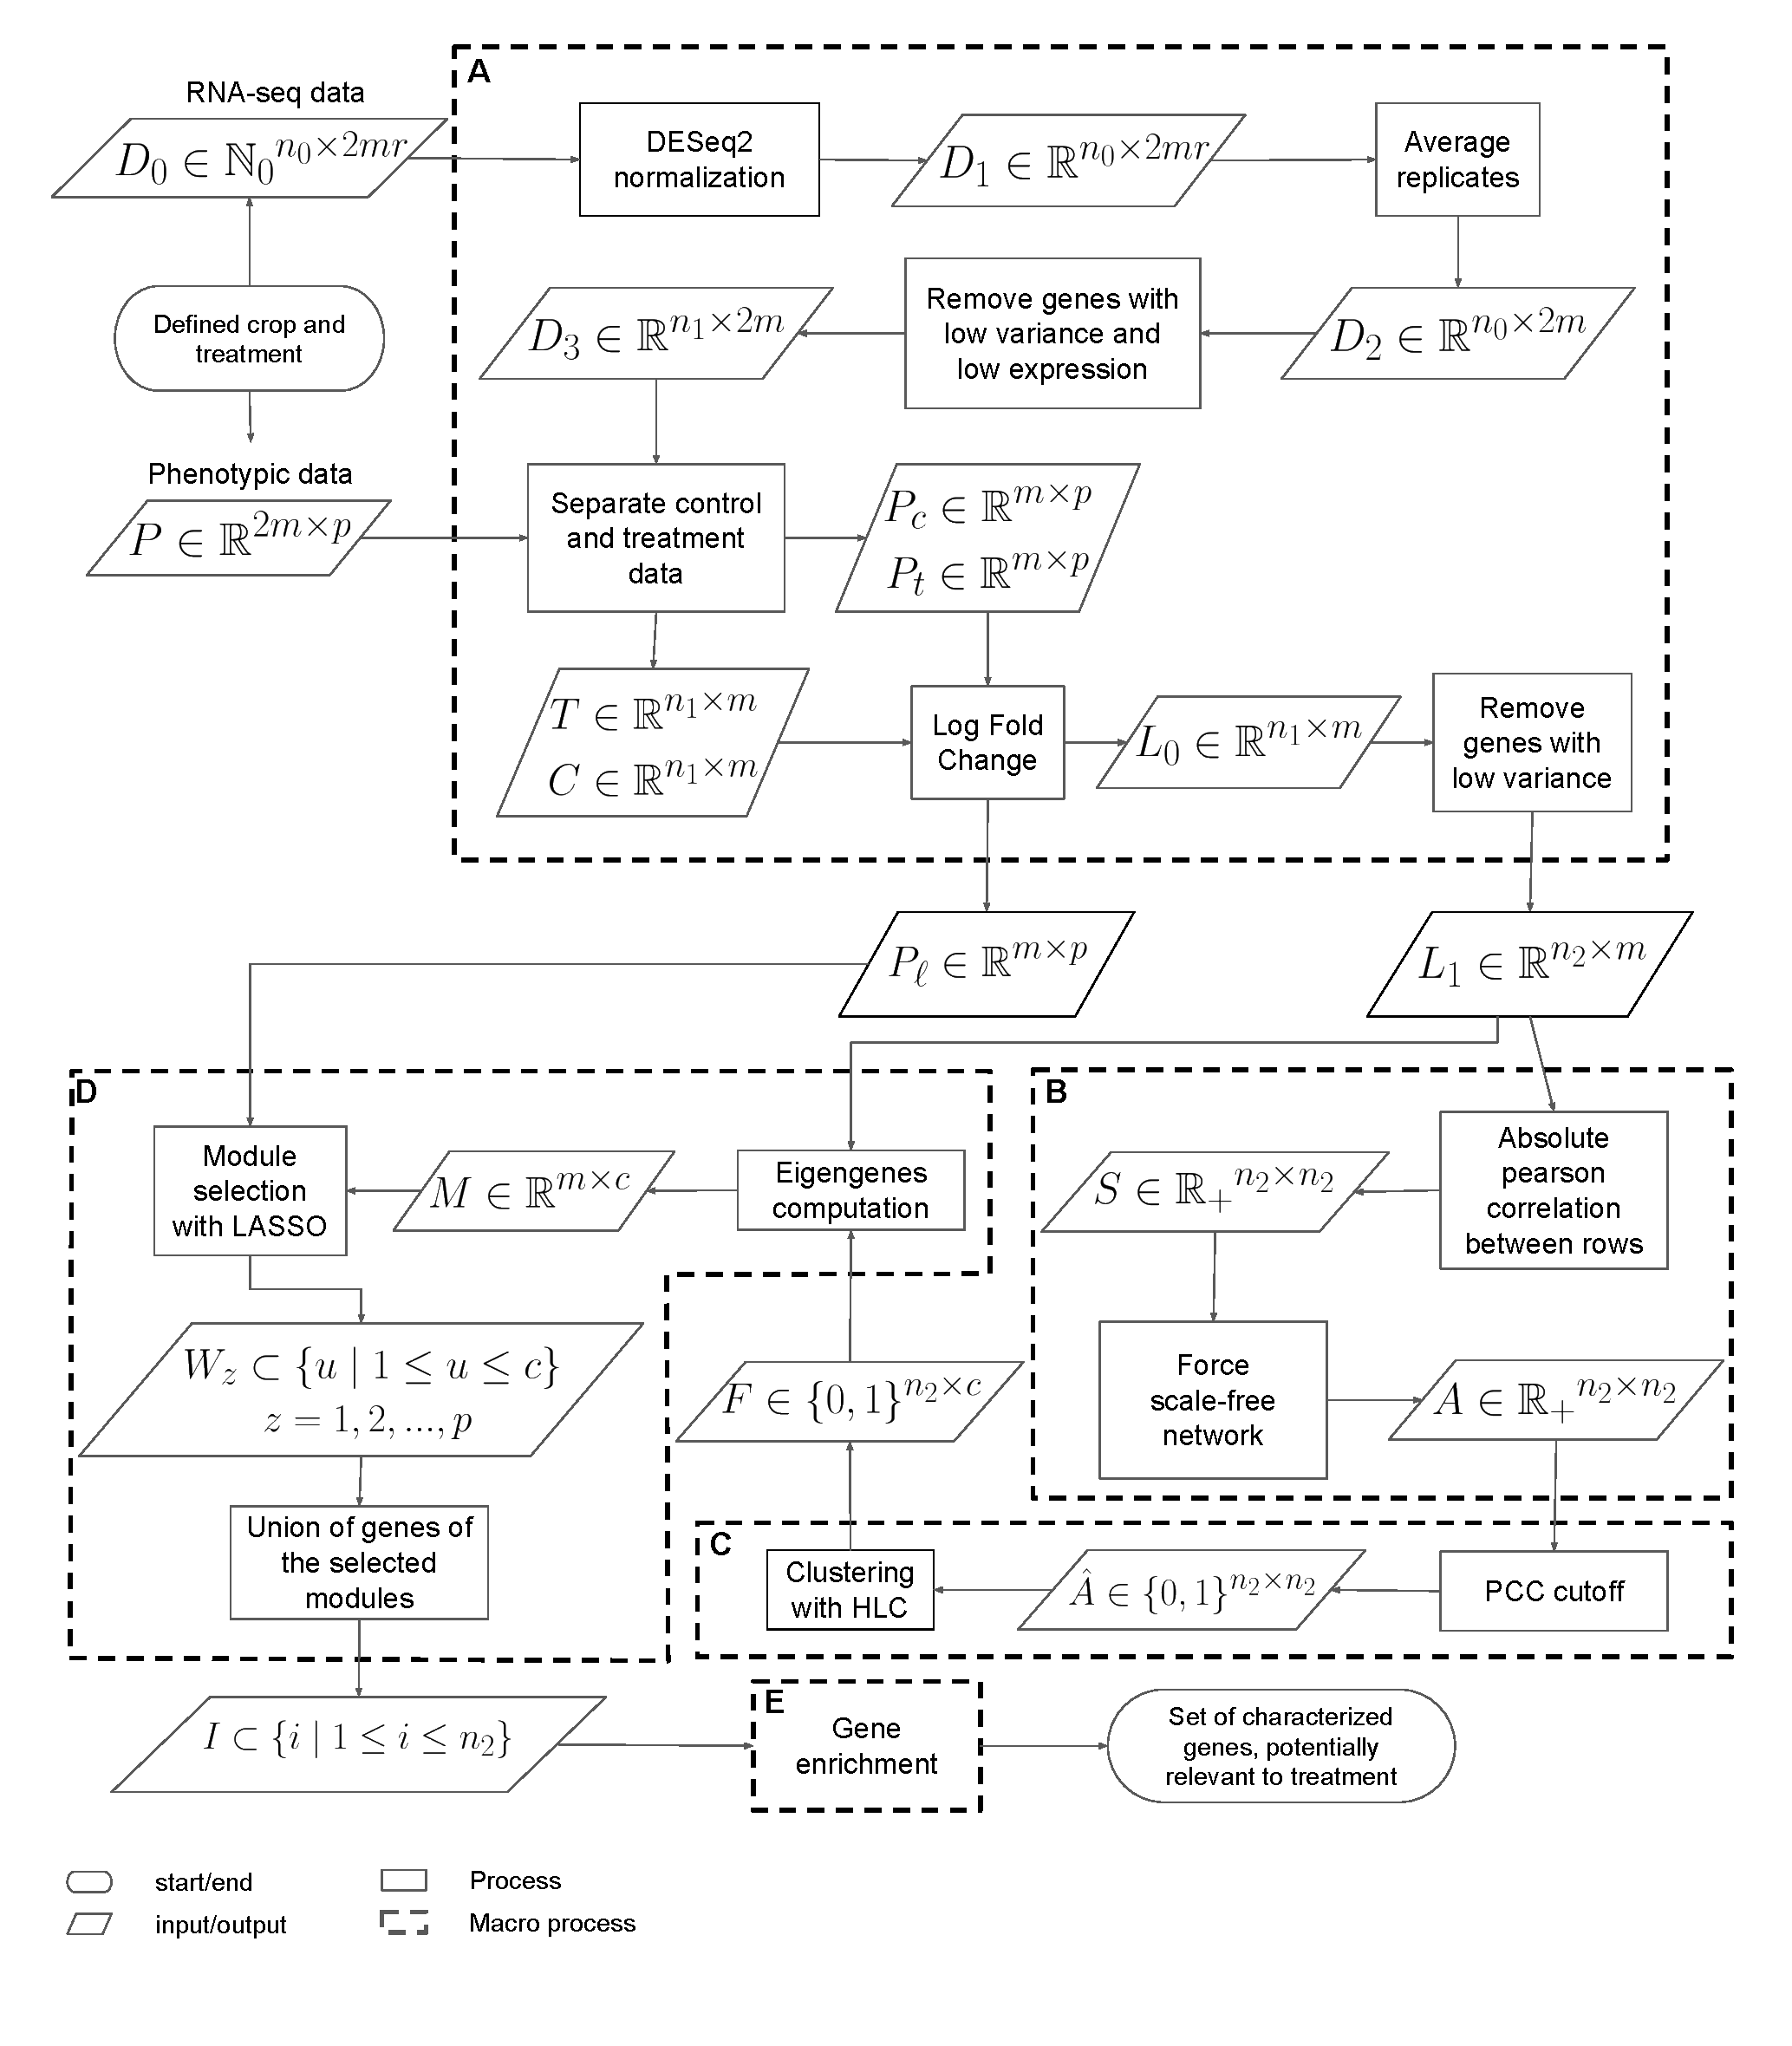
\includegraphics[clip,width=0.96\textwidth]{figures/figure1.pdf}
  \caption[The proposed workflow comprising five macro-steps]%
  {The proposed workflow comprising five macro-steps:
    A.~Data pre-processing, B.~Co-expression network
    contruction, C.~Co-expression module identification,
    D.~Modules association to phenotypic traits, and
    E.~Gene enrichment.}
  \label{fig:flow_chart}
\end{figure}

The workflow uses RNA-seq read counts, representing gene expression
levels, as input data. More precisely, it uses $n_0$ gene expression
profiles of an organism, measured for $m$ different genotypes under
control and treatment conditions, and $r$ biological replicates. This
raw data is represented as a matrix $D_0 \in {\mathbb{N}_0}^{n_0
  \times 2mr}$. In order to discover key genes and their interaction
with phenotypes related to treatment tolerance, the approach also
requires a set of $p$ phenotypic traits, measured for the $m$
genotypes. The phenotypic data is seen as a matrix $P \in
\mathbb{R}^{2m \times p}$ containing two phenotypic values per
genotype, one under control condition and a second one under treatment
condition.

\subsection*{Data Pre-processing}

The goal of the data pre-processing stage is to build matrices
$P_\ell$ and $L_1$ representing, respectively, the changes in
phenotypic values and expression levels between control and treatment
condition, from RNA-seq and phenotypic data found in matrices $D_0$
and $P$, respectively.
\vspace{0.5cm}

The RNA-seq data cannot be directly interpreted. Therefore, a
normalization process is applied to deal with the problem of possible
biases affecting the quantification of results. The suggested
normalization technique for correcting library size and RNA
composition bias is DESeq2~\cite{love2014moderated}. The normalized
data is represented as a matrix $D_1 \in \mathbb{R}^{n_0 \times 2mr}$,
and the biological replicates of each genotype are averaged and
represented as a matrix $D_2 \in \mathbb{R}^{n_0 \times 2m}$. The
genes exhibiting low variance or low expression are removed from
$D_2$, thus identifying a subset of size $n_1 \leq n_0$ of the
original genes. The control and treatment data is separated into the
matrices $C\in \mathbb{R}^{n_1 \times m}$ and $T\in \mathbb{R}^{n_1
  \times m}$, respectively. The matrix entries $c_{ij}$ in $C$ and
$t_{ij}$ in $T$ represent the normalized expression
level of gene $i$ in accession $j$ under control and treatment 
condition, respectively.
Control and treatment data is also separated from
phenotypic data $P$, obtaining the $P_c$ and $P_t$ matrices of
dimensions $m \times p$.
\vspace{0.5cm}

In the above configuration, the changes in expression levels and
phenotypic values between control and treatment conditions, are
measured in terms of logarithmic ratios. In the case of expression
levels, the log ratios are represented in the Log Fold Change matrix
$L_0 \in \mathbb{R}^{n_1 \times m}$, where $\ell_{ij}=\log_2
(t_{ij}/c_{ij})$. Similarly, the log ratios of the phenotypic data are
computed and represented in the $P_\ell \in \mathbb{R}^{m \times p}$
matrix.
\vspace{0.5cm}

The final step of the data pre-processing is to filter $L_0$ by
removing rows (e.g., genes) with low variance in the differential
expression patterns, obtaining a new matrix $L_1$ of dimensions $n_2
\times m$, with $n_2 \leq n_1$.

\subsection*{Co-expression Network Construction}

A gene co-expression network connect genes with similar expression
patterns across biological conditions. The purpose of this stage is to
describe how to build the co-expression network $A$ from the Log Fold
Change matrix $L_1$, capturing the relationship between genes
according to the change in expression levels between the two studied
conditions. These co-expression patterns are meaningful for the
identification of genes not yet associated with the response to the
treatment condition.
\vspace{0.5cm}

The Log Fold Change matrix $L_1$ is used to build the co-expression
network following the first two steps of the WGCNA
methodology~\cite{langfelder2008wgcna}. First, the level of
concordance between gene differential expression profiles across
samples is measured. To this end, the absolute value of the Pearson
correlation coefficient is used as the similarity measure between
genes and the resulting values are stored in the similarity matrix
$S\in \mathbb{R_{+}}^{n_2 \times n_2}$. Second, the matrix $S$ is
transformed into an adjacency matrix $A \in \mathbb{R_+}^{n_2\times
  n_2}$ where each entry $a_{ij} = (s_{ij})^\beta $ encodes the
connection strength between each pair of genes. In other words, the
elements of the adjacency matrix are the similarity values up to the
power $\beta > 1$ so that the degree distribution will fit a
scale-free network. These networks contain many nodes with very few
connections and a small number of hubs with high connections. In a
strict scale-free network, the logarithm of $P(k)$ (i.e., the
probability of a node having degree $k$) is approximately inversely
proportional to the logarithm of $k$ (i.e., the degree of a node).
The parameter $\beta$ is chosen to be the smallest power such that the
$R^2$ of the linear regression between $log_{10}(p(k))$ and
$log_{10}(k)$ is close to $1$ (e.g., $R^2 > 0.85$).

\subsection*{Co-expression Module Identification}

The next step in the workflow is to identifying communities (also
called modules) from the co-expression network structure and dynamics
represented in $A$.  The idea is to cluster genes with similar
patterns of differential expression change. Membership in these
modules may overlap in biological contexts, because modules may be
related to specific molecular, cellular, or tissue functions, and the
biological components (i.e., genes) may be involved in multiple
functions. Thus, unlike WGCNA, the adjacency matrix $A$ is used to
detect overlapping (rather than non-overlapping) communities, using
the Hierarchical Link Clustering (HLC) algorithm (see
%Section~\ref{sec.prelim}).
\hyperref[sec.prelim]{Preliminaries}).
\vspace{0.5cm}

As a preliminary step, matrix $A$ is transformed into an unweighted
network $\hat{A} \in \{0,1\}^{n_2 \times n_2}$ before using the
clustering algorithm. To this end, the Pearson Correlation Coefficient
(PCC) cutoff is determined using the approach described
in~\cite{aoki2007approaches}. The number of nodes, edges, and the
network density is determined for different PCC cutoffs. Near the most
biological relevant PCC cutoff, the number of nodes presents a linear
decrease and the density of the network reaches its minimum, while
below this value the number of edges rapidly increases. Following this
observation, a cutoff is selected such that gene pairs which have a
correlation score higher than the threshold are considered to have
important co-expression relationship. Above the cutoff, the entries of
matrix $A$ become $1$ and below the cutoff $A$ values become $0$. The
HLC algorithm organizes the $n_2$ genes of matrix $\hat{A}$ into $c$
modules, where each gene can belong to zero, one or multiple modules.
This information is represented as an affiliation matrix $F \in
\{0,1\}^{n_2 \times c}$, where $f_{iu} = 1$ iff node $i$ is member of
module $u$ (it is 0, otherwise).

\subsection*{Module Association to Phenotypic Traits}

To identify the most relevant modules of genes, associated
with the phenotypic response to a specific treatment in an organism,
the proposed workflow uses LASSO. Specifically, each module is
represented by an eigengene, which is defined as the first principal
component of such module. An eigengene can be seen as an average
differential expression profile for each community: it is computed
from the Log Fold Change Matrix $L_1$ and the affiliation matrix
$F$. Given a module $u$, the affiliation matrix is used to identify
the genes belonging to $u$ and then the corresponding rows of the
matrix $L_1$ are selected to compute the first principal component of
$u$. Each principal component becomes a column of the matrix $M \in
\mathbb{R}^{m \times c}$.  These profiles are then associated with each
phenotypic trait using
LASSO.  In this context, the eigengenes (i.e., the columns
of $M$) act as regressor variables and each phenotypic trait (i.e.,
each column of $P_\ell$) is used as an outcome variable.
\vspace{0.5cm}

The output after applying LASSO is a set $W_z$ of modules for each
phenotypic trait $z$, where $W_z \subset \{u \mid 1 \leq u \leq c\}$
for $z= 1,2,..,p$. The target genes $I$ for downstream analysis, which
may be important in the treatment response, are the union of genes
belonging to the selected modules; that is $I = \cup_{z=1}^{p} W_z$,
where $I \subset \{i \mid 1 \leq i \leq n_2\}$.

\subsection*{Gene Enrichment}

The goal of this final stage of the process is to annotate with
additional information the genes identified in previous stages,
helping to elucidate their possible behavior and role in the response
to the studied treatment.
\vspace{0.5cm}

A crucial step is to identify the differentially expressed genes in
set $I$. That is, to select those genes in $I$ having an absolute
value of the Log Fold Change of at least $2$ ($|\ell_{ij}|\geq 2$) for
at least one sample. This represents genes whose expression level is
quadrupled (up or down) from control to treatment condition; they are the
strong candidates for treatment responsive genes.
\vspace{0.5cm}

Also, functional category enrichment can be done by, e.g., searching
for gene ontology annotations in databases such as
QuickGO~\cite{binns2009quickgo}. Such annotations can provide evidence
of biological implications of the target genes in the
treatment-tolerance mechanisms. Furthermore, QuickG0 can be used to
identify genes with reported protein products, which can be used to
perform additional relevant analysis reviewing their reported
protein-protein interactions in other databases, such as
STRING~\cite{szklarczyk2016string}. The interactions include direct
(physical) and indirect (functional) associations, and they stem from
computational prediction, knowledge transfer between organisms, and
interactions aggregated from other (primary) databases. This
information can give new insights on how the selected genes are
involved in functional pathways that can be related to the treatment
of interest.

%\section*{Results}
\section*{Identifying Potential Saline Stress Responsive Genes in Rice}
\label{sec.case}

This section presents a case study on the identification of genes in
\textit{Oryza sativa} that may respond to saline stress following the
approach presented in %Section~\ref{sec.framework}.
\hyperref[sec.framework]{The Workflow}.
\vspace{0.5cm}

The RNA-seq data used for the experiments summarized in this section
was obtained from GEO database \cite{clough2016gene} (accession
number GSE98455). This data corresponds to $n_0=57\,845$ gene
expression profiles of shoot tissues measured for both control and
salt condition in $m=92$ accessions of the Rice Diversity Panel 1~\cite{eizenga2014registration},
with $r=2$ biological replicates. A total of $p=3 $ phenotypic traits
are used: shoot $K^+$ content, root biomass, and shoot biomass. These
traits were measured for the same $92$ genotypes, under control and
salt stress conditions, and can be found in the supplementary
information of~\cite{campbell2017allelic}.

\subsection*{Data Pre-processing}

DESeq2 normalization is applied to the raw data and the biological
replicates are averaged. Genes exhibiting low variance are
identified as those with ratio of upper quantile to lower quantile
smaller than $1.5$ and are removed from the normalized data. Genes
with low expression, corresponding to those having more than $80\%$
samples with values smaller than $10$, are also removed. A total of
$n_1 = 9\,414$ genes are kept after this filtering process.
\vspace{0.5cm}

From the Log Fold Change matrix $L_0$, genes whose difference between
upper quantile and lower quantile greater than $0.25$ are
removed. Therefore, the resulting matrix $L_1$ contains the log ratios
of $n_2 = 8\,928$ genes. The logarithmic ratios of the phenotypic data,
for the $92$ accessions and the $3$ traits, are also computed.

\subsection*{Co-expression Network Construction}

The Log Fold Change matrix $L_1$ is used to compute the corresponding
similarity matrix.  For this network, it is observed that $\beta=3$ is
the smallest integer such that the $R^2 \geq 0.8
$. Figure~\ref{fig:beta} depicts the degree distribution of the
similarity matrix (left) and the degree distribution of the adjacency
matrix (right), which is the degree distribution of a scale-free
network with $R^2 = 0.8$ with $\beta = 3$.
\vspace{0.5cm}

%figure 2
\begin{figure}[htbp]
  \centering
    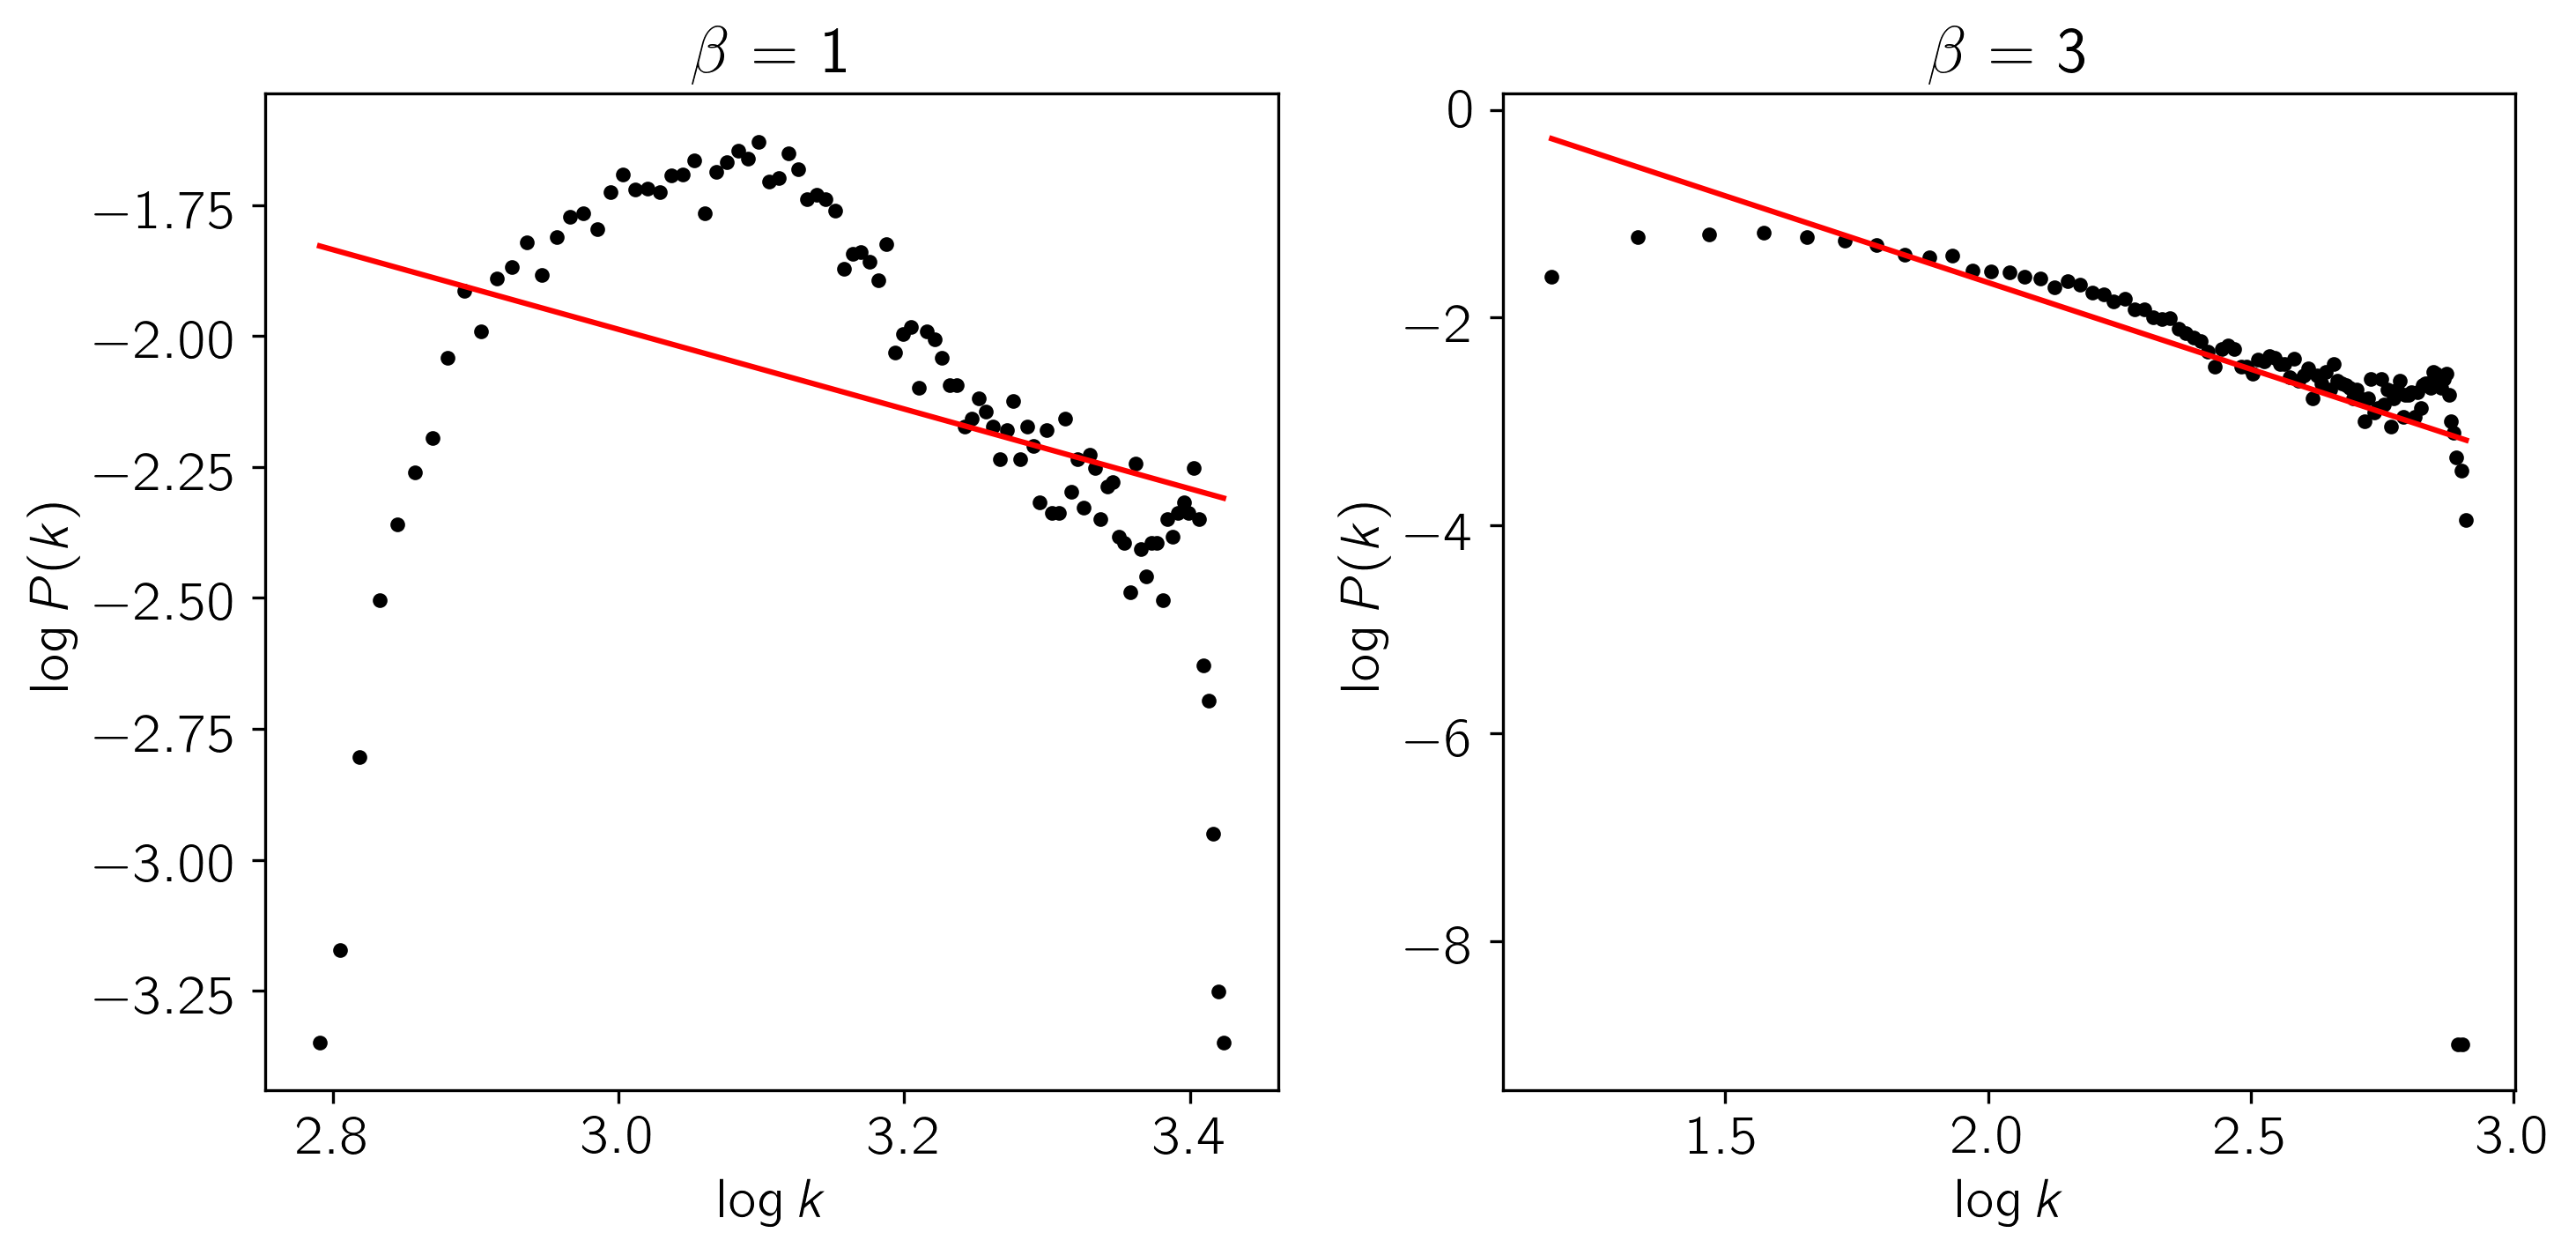
\includegraphics[clip,width=0.8\textwidth]{figures/figure2.png}
  \caption{Degree distribution of $A$ (left) and $\hat{A}$ (right).}
  \label{fig:beta}
\end{figure}

The resulting adjacency matrix $A$ represents a complete graph
$G=(V,E)$, with $|V| = 8\,928$ genes ($|E| = 39\,850\,128$ edges).

\subsection*{Co-expression Module Identification}

The adjacency matrix $A$ is transformed into an unweighted network
$\hat{A}$ applying the approach described
in~\cite{aoki2007approaches}. The cutoff value is set to $0.2$, 
based on the density of the network
combined with the decreasing number of nodes and edges with higher PCC
values. Thus keeping only the
connections above this threshold and removing the isolated nodes. The
resulting adjacency matrix $\hat{A}$ has $5\,810$ connected genes and
accounts for $16\,875\,145$ edges.
\vspace{0.5cm}

After applying the HLC algorithm, a total of $4\,131$ genes are
distributed in $c = 5\,143$ overlapping modules of at least $3$
genes. Figure~\ref{fig:overlap} presents a histogram of the
overlapping percentage of these genes, measured as the proportion of
modules to which each gene belongs. The first bar of the histogram
represents the genes with zero overlap, corresponding to $28\%$ of the
total genes; the remaining $72\%$ represents the genes belonging to
more than one module.

%figure 3
\begin{figure}[htbp]
  \centering
    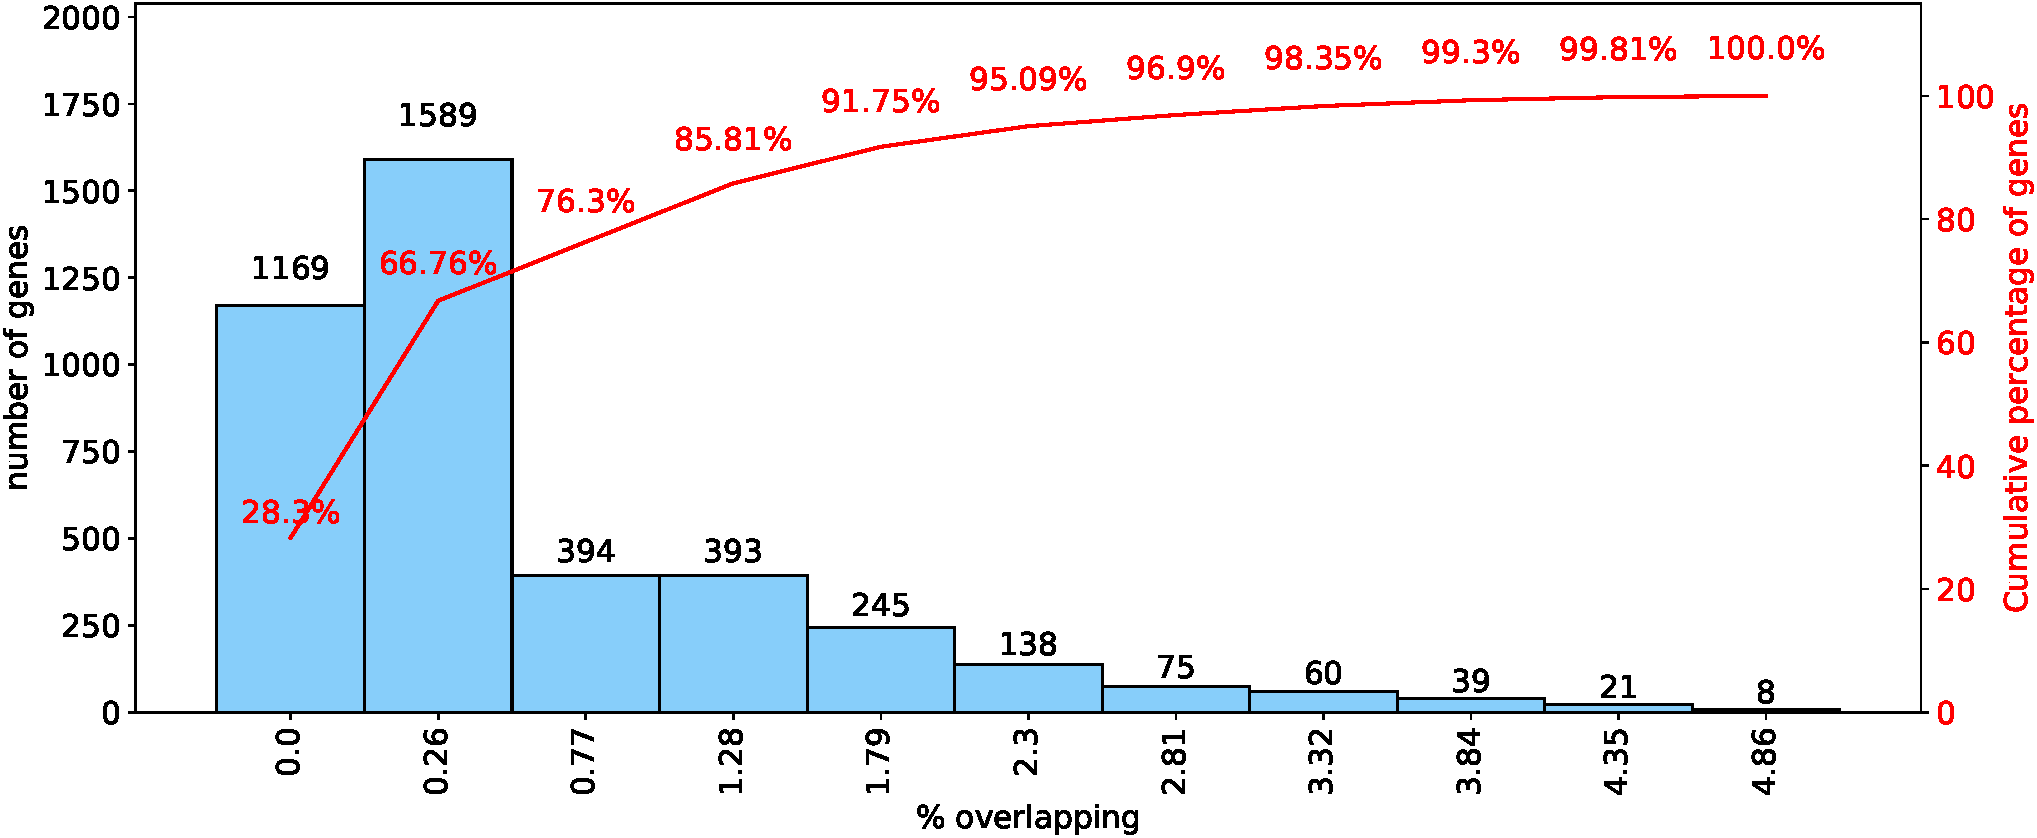
\includegraphics[clip,width=0.5\textwidth]{figures/figure3.png}
  \caption{Overlapping percentage of genes after applying HLC.}
  \label{fig:overlap}
\end{figure}

\subsection*{Module Association to Phenotypic Traits}

The phenotypic traits under study are shoot $K^+$ content, root
biomass, and shoot biomass. Figure~\ref{fig:pdata} suggests that there
are significant differences in the values of these phenotypic traits
between stress and control conditions. This supports the working
hypothesis that these three variables represent tolerance-associated
traits in rice under salt stress.
\vspace{0.5cm}

%figure 4
\begin{figure}[htbp]
  \centering
    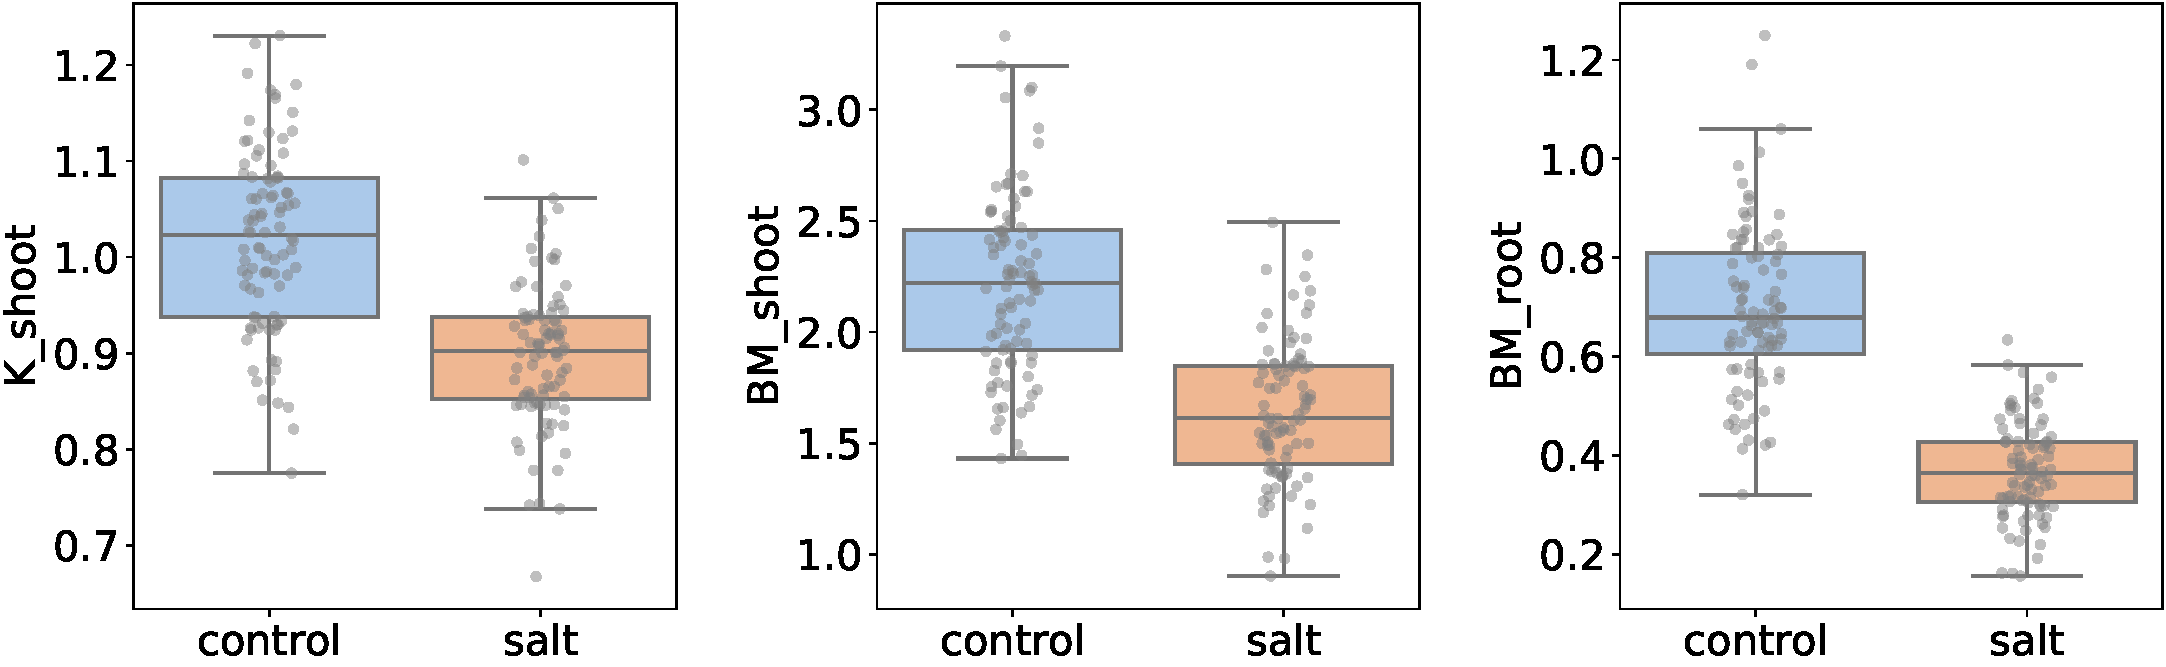
\includegraphics[clip,width=0.9\textwidth]{figures/figure4.png}
  \caption{Phenotipic traits distribution under control and salt stress.}
  \label{fig:pdata}
\end{figure}

Using the affiliation matrix $F$ derived from the HLC output and the
Log Fold Change matrix $L_1$, a matrix $M$ is built by computing the
eigengene for each of the $c = 5\,143$ modules. The LASSO technique is
applied by using each of the phenotypic traits as the outcome
variable, one at a time. As shown in Figure~\ref{fig:cross-val},
cross-validation is performed for each phenotypical trait in order to
select the corresponding regularization parameter $\lambda$ that
minimizes the mean-squared error.
\vspace{0.5cm}

%figure 5
\begin{figure}[htbp]
  \centering
    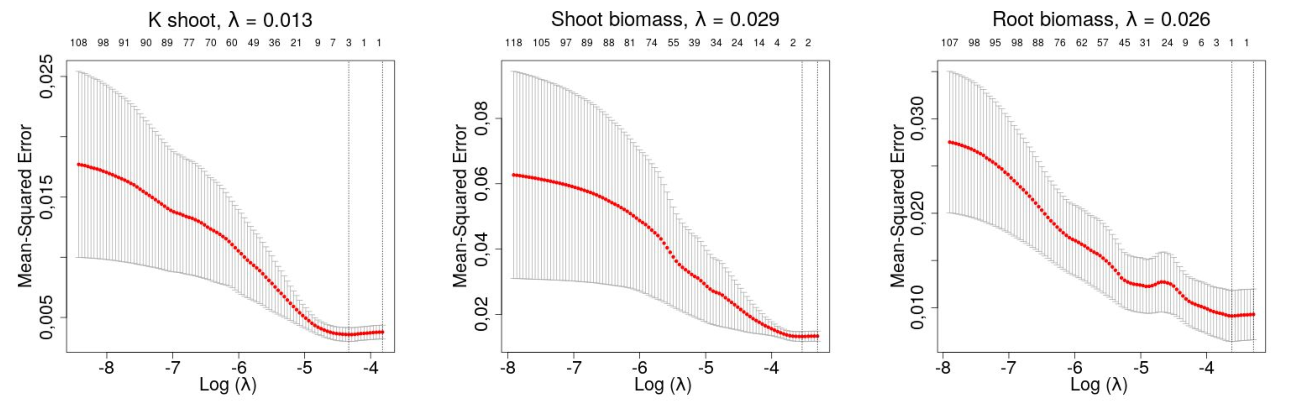
\includegraphics[clip,width=0.96\textwidth]{figures/figure5.pdf}
  \caption{Cross-validation of the LASSO regularization parameter
    $\lambda$, for each phenotypic trait.}
  \label{fig:cross-val}
\end{figure}

Finally, three LASSO models are adjusted by using the corresponding
$\lambda$ and phenotypical data with the eigengenes of matrix $M$. As
result, 6 modules are detected as relevant in the response to salt
stress in rice: 3 modules of 3 genes, each associated with shoot $K$
content; 2 modules of 3 genes associated with shoot biomass; and 1
module of 4 genes associated with root biomass (see
Figure~\ref{fig:final_genes}).

\subsection*{Gene Enrichment}

From the $19$ genes selected by LASSO, all but $3$ genes (the ones
associated to $K$ content), are also identified as deferentially
expressed ($|\ell_{ij}| \geq 2$) for at least one of the $92$
accessions. This suggests that those genes are strong candidates as
stress responsive genes to salt conditions in rice.
\vspace{0.5cm}

Figure~\ref{fig:final_genes} summarizes how from the initial
$n_0=57\,845$ genes, the proposed workflow identifies a reduced set of
$19$ genes. First, $48\,431$ genes are discarded after filtering the
normalized expression data $D_2$ and then $486$ additional genes are
discarded when filtering the Log Fold Change matrix $L_0$, to finally
arrive at $19$ genes, of which $16$ are differentially expressed.
\vspace{0.5cm}

% figure 6
\begin{figure}[htbp]
  \centering
    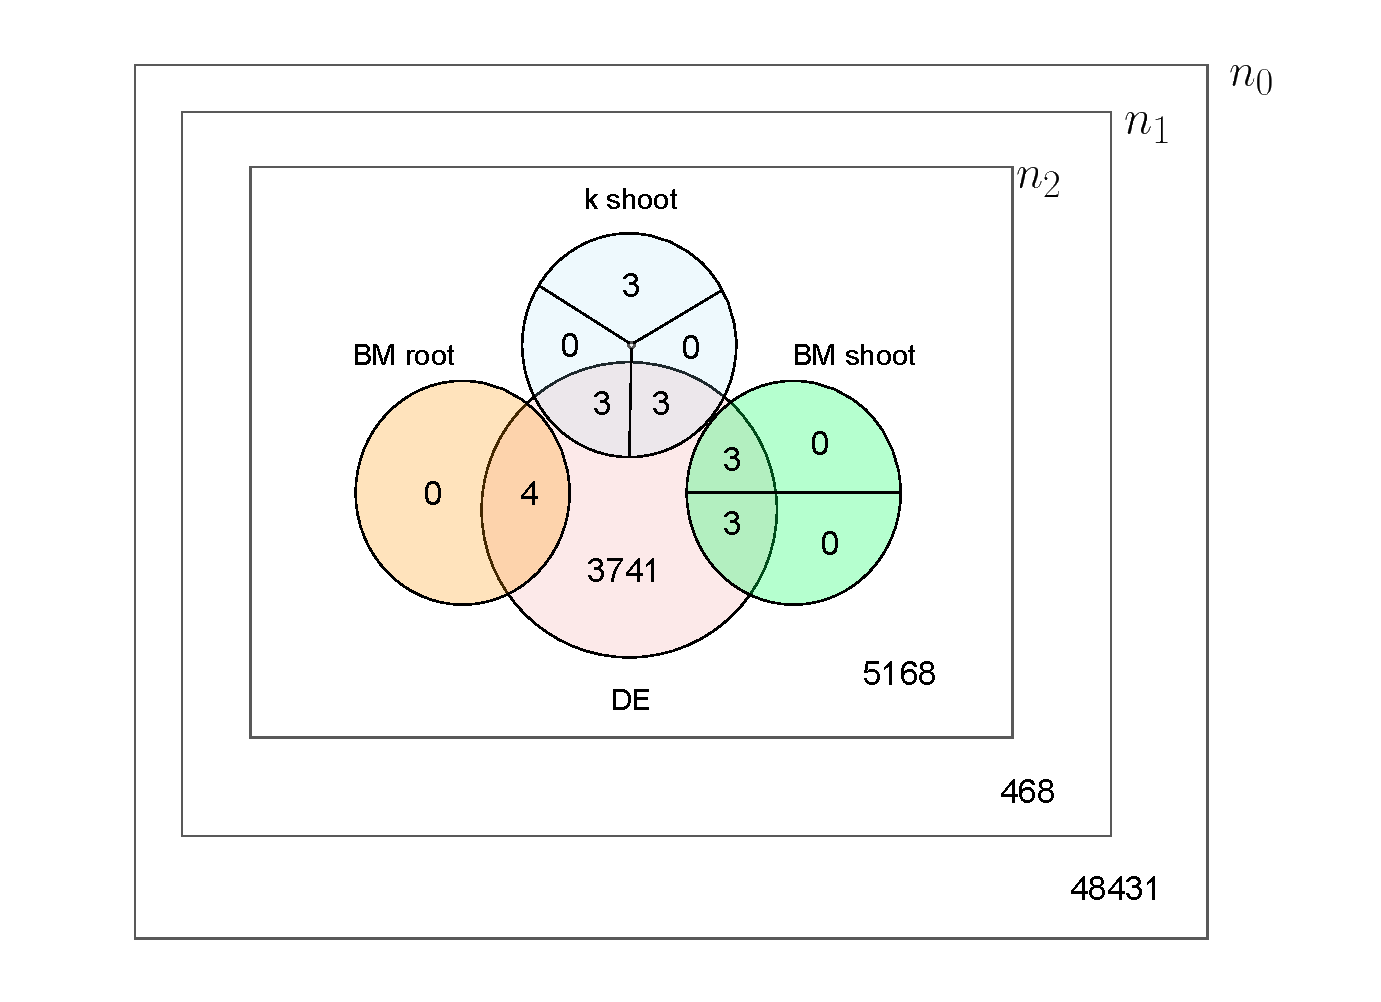
\includegraphics[clip,width=0.8\textwidth]{figures/figure6.pdf}
   \caption[Venn diagram for the case study in rice]%
   {Venn diagram representing the number of genes selected at
    different stages of the proposed workflow for the case study in
    rice.}
  \label{fig:final_genes}
\end{figure}

According to the Quickgo database, only $2$ of the $16$ differentially
expressed genes (both from the module related to shoot biomass) are
named and have an associated protein product: spermidine
hydroxycinnamoyltransferase 2 (SHT2) and lipoxygenase.
Figure~\ref{fig:3d} shows their corresponding 3D protein structures.
\vspace{0.5cm}

%figure 7
\begin{figure}[htbp]
  \centering
    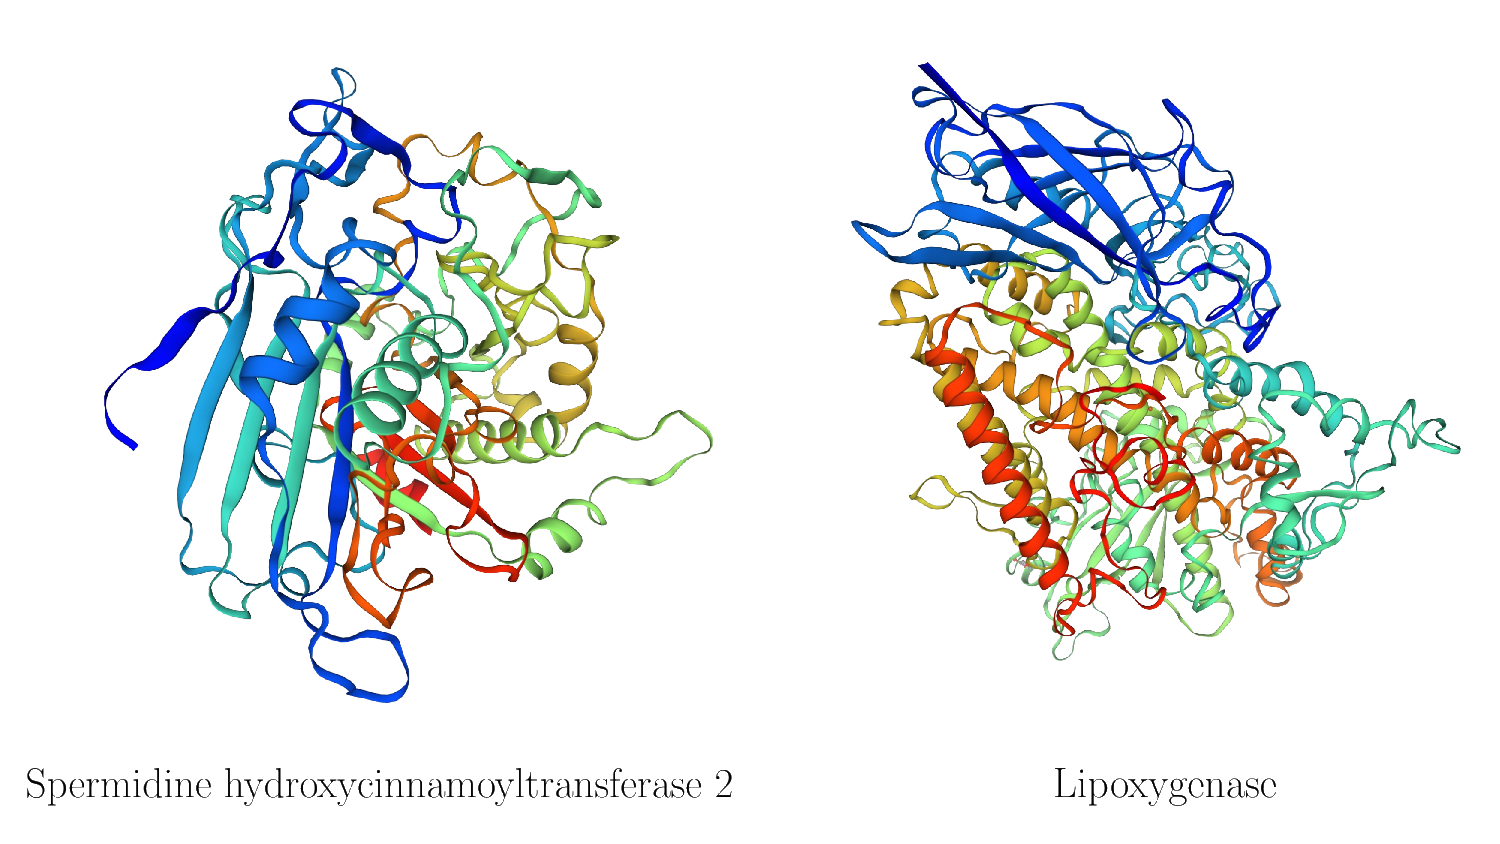
\includegraphics[clip,width=0.8\textwidth]{figures/figure7.pdf}
  \caption{3D protein structure of named genes selected by LASSO, borrowed from~\cite{szklarczyk2016string}.}
  \label{fig:3d}
\end{figure}

The Uniprot database~\cite{uniprot2018uniprot} reports, on the one
hand, that SHT2 contributes to the natural variation of
spermidine-based phenolamides in rice cultivars. On the other hand, it
is reported in~\cite{uniprot2018uniprot} that plant lipoxygenase may
be involved in a number of diverse aspects of plant physiology
including growth and development, pest resistance, and senescence or
responses to wounding. This protein is involved in the pathway
oxylipin biosynthesis, which is part of Lipid metabolism. Additionally,
previous studies
%
in~\cite{gupta2013plant,hou2015persimmon,mittova2002salt,peng2019novel,roychoudhury2011amelioration}
%
provide evidence of biological implications of sperimidine and
lipoxygenase in tolerance to salt stress in other plants or even in
rice cultivars.

As a conclusion, the results presented in this section suggest that
further studies are needed to elucidate the detailed biological
function of the remaining 14 genes that have not been named so far in
the literature.  They may have the potential to intervene in stress
responsive mechanisms to salt conditions in rice.


\section*{Concluding Remarks}
\label{sec.concl}

This manuscript provides a detailed description of a network-based
analysis workflow for the discovery of key genes responding to a
specific treatment in an organism. It links transcriptomic with
phenotypic data and identifies overlapping gene modules.
\vspace{0.5cm}

The proposed approach is inspired by the workflow suggested in the
WGCNA~\cite{langfelder2008wgcna}. Its main steps are the preprocessing
of the gene expression data, the construction of a co-expression
network, the detection of modules within the network, the relation of
modules with external information (e.g., phenotypic data), and the
enrichment of the identified key genes with additional information.
Both approaches are structured in a modular way, which allows
modifying and exploring different techniques in each step of the
workflow.
\vspace{0.5cm}

The proposed workflow is designed to integrate expression data
measured under two different conditions (namely, control and
treatment), unlike the usually co-expression-based approaches which
work with both conditions independently or consider only a single
condition. For this purpose, an approach similar to that proposed
in~\cite{du2019network} is used, where the control and treatment data
are compiled in a single matrix using the Log Fold Change
measure. Thus, the input to construct the co-expression network is not
the expression data, but instead the changes in the expression levels
from one condition to the other, making room for capturing the signal
of changes caused by the treatment.
\vspace{0.5cm}

An important feature in the proposed workflow is the module
detection technique. The co-expression network is computed, as in
WGCNA, until a scale-free network is obtained. In the proposed
approach, this network is then used to apply the HLC algorithm, a
clustering technique capable of detecting overlapping
communities. Several approaches of module detection from gene
expression have been proposed and were evaluated
in~\cite{saelens2018comprehensive}. Most of them focus mainly on
disjoint (non-overlapping) communities; the techniques described
dealing with overlaps are not clustering, but bi-clustering and
decomposition methods. It is well known that communities in real
networks, including biological ones, are likely
overlap~\cite{palla2005uncovering}. Thus, the approach presented
in this work can be seen as a generalization of the previous
approaches, such as WGCNA, with the potential to deal with genes
associated to multiple biological processes.
\vspace{0.5cm}

The approach was applied in a case study with rice under salt
stress. The results show a group of 14 genes, of which only $2$ of
them have been previously related to saline stress response in other
studies. As future work, other overlapping module detection and
selection techniques should be used instead HLC and LASSO,
respectively. The combination of these techniques would allow finding
target genes for future biological studies that evaluate their
potential as genes that respond to salt stress in rice, and other
crops and stresses. In-vivo laboratory experimentation needs to be
conducted to validate the findings of this paper in relation to
salinity stress.
\vspace{0.5cm}

Finally, the workflow is presented as a protocol capable of
considerably reducing the number of genes detected as relevant in the
response to stress of choice. Other traditionally used methods for
this purpose tend to generate a large list of candidate genes, thus
limiting subsequent efforts in experimental validation. In this sense,
the proposed workflow can help in reducing such efforts in time and
money invested by researchers in the experimental validation of
stress-responsive genes.


%\section*{Appendix}
%Text for this section\ldots

%%%%%%%%%%%%%%%%%%%%%%%%%%%%%%%%%%%%%%%%%%%%%%
%%                                          %%
%% Backmatter begins here                   %%
%%                                          %%
%%%%%%%%%%%%%%%%%%%%%%%%%%%%%%%%%%%%%%%%%%%%%%


\begin{backmatter}

\section*{Acknowledgements}%% if any
Not applicable

\section*{Funding}%% if any
This work was funded by the OMICAS program: Optimización Multiescala In-silico de
Cultivos Agrícolas Sostenibles (Infraestructura y Validación en Arroz y Caña de Azúcar),
anchored at the Pontificia Universidad Javeriana in Cali and funded within the Colombian
Scientific Ecosystem by The World Bank, the Colombian Ministry of Science, Technology and
Innovation, the Colombian Ministry of Education and the Colombian Ministry of Industry 
and Turism, and ICETEX, under GRANT ID: FP44842-217-2018.

\section*{Abbreviations}%% if any
\textbf{HLC:} Hierarchical Link Clustering\\
\textbf{LASSO:} Least Absolute Shrinkage Selector Operator\\
\textbf{PCC:} Pearson Correlation Coefficient\\
\textbf{RNA-seq:} RNA sequencing\\
\textbf{SHT2:} Spermidine hydroxycinnamoyltransferase 2\\
\textbf{WGCNA:} Weighted Gene Co-expression Network Analysis\\

\section*{Availability of data and materials}%% if any
The datasets analysed during the current study are publicy available. They can be found in the following locations:
\begin{itemize}
\item RNA-seq data of salt stress in rice is available on the GEO (GSE98455).
\item Phenotypic data of salt stress in rice is a subset of the supplementary file 1 included in ~\cite{campbell2017allelic}.
\end{itemize}

\section*{Ethics approval and consent to participate}%% if any
Not applicable

\section*{Competing interests}
The authors declare that they have no competing interests.

\section*{Consent for publication}%% if any
Not applicable

\section*{Authors' contributions}
J.F. and C.R. proposed the original idea. 
J.F. provide advice on algorithms concepts and implementation.
C.R. structured the methodology and performed the analysis. 
C.R., J.F., and H.C.R. wrote the manuscript.
All authors read and approved the final manuscript.


%%%%%%%%%%%%%%%%%%%%%%%%%%%%%%%%%%%%%%%%%%%%%%%%%%%%%%%%%%%%%
%%                  The Bibliography                       %%
%%                                                         %%
%%  Bmc_mathpys.bst  will be used to                       %%
%%  create a .BBL file for submission.                     %%
%%  After submission of the .TEX file,                     %%
%%  you will be prompted to submit your .BBL file.         %%
%%                                                         %%
%%                                                         %%
%%  Note that the displayed Bibliography will not          %%
%%  necessarily be rendered by Latex exactly as specified  %%
%%  in the online Instructions for Authors.                %%
%%                                                         %%
%%%%%%%%%%%%%%%%%%%%%%%%%%%%%%%%%%%%%%%%%%%%%%%%%%%%%%%%%%%%%

% if your bibliography is in bibtex format, use those commands:
\bibliographystyle{bmc-mathphys} % Style BST file (bmc-mathphys, vancouver, spbasic).
\bibliography{biblio}      % Bibliography file (usually '*.bib' )
% for author-year bibliography (bmc-mathphys or spbasic)
% a) write to bib file (bmc-mathphys only)
% @settings{label, options="nameyear"}
% b) uncomment next line
%\nocite{label}

% or include bibliography directly:
% \begin{thebibliography}
% \bibitem{b1}
% \end{thebibliography}

%%%%%%%%%%%%%%%%%%%%%%%%%%%%%%%%%%%
%%                               %%
%% Figures                       %%
%%                               %%
%% NB: this is for captions and  %%
%% Titles. All graphics must be  %%
%% submitted separately and NOT  %%
%% included in the Tex document  %%
%%                               %%
%%%%%%%%%%%%%%%%%%%%%%%%%%%%%%%%%%%

%%
%% Do not use \listoffigures as most will included as separate files

%\section*{Figures}
%
%%flow chart
%\begin{figure}[h!]
%  \centering
%    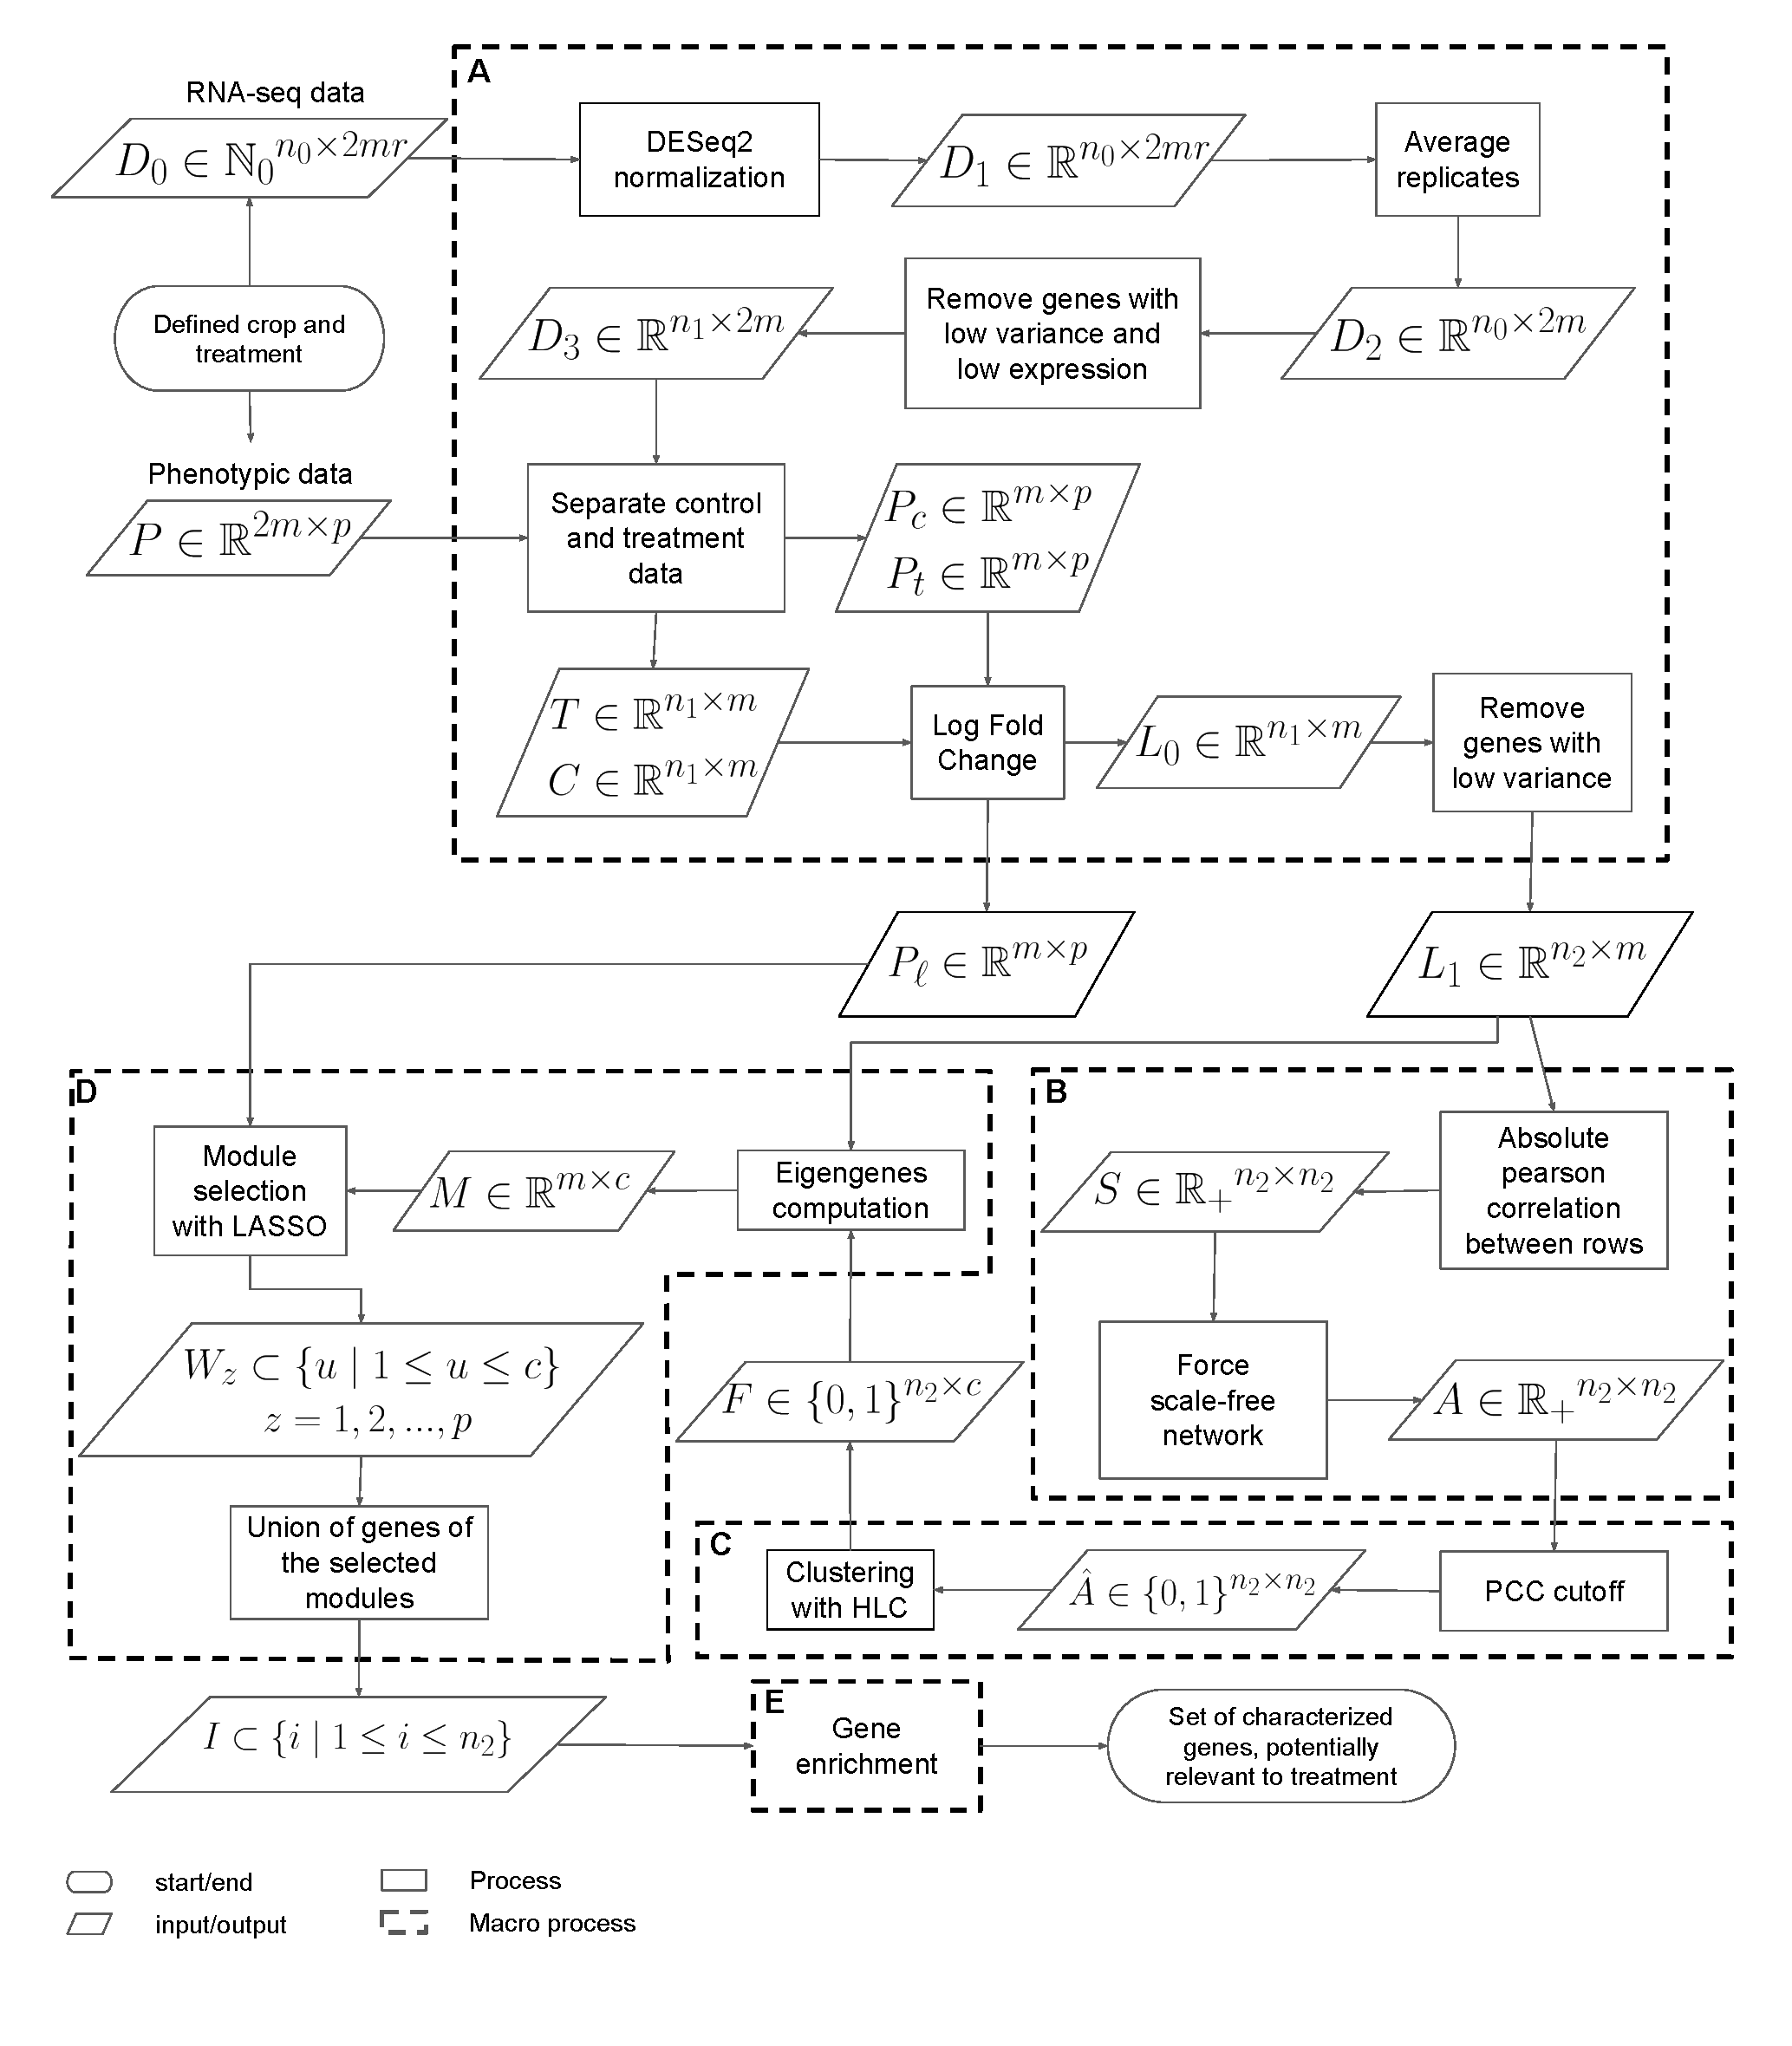
\includegraphics[clip,width=1\textwidth]{figures/figure1.pdf}
%  \caption[The proposed workflow comprising five macro-steps]%
%  {The proposed workflow comprising five macro-steps:
%    A.~Data pre-processing, B.~Co-expression network
%    contruction, C.~Co-expression module identification,
%    D.~Modules association to phenotypic traits, and
%    E.~Genes enrichment.}
%  \label{fig:flow_chart}
%\end{figure}
%
%%scale-free beta 1 y 3
%\begin{figure}[h!]
%  \centering
%    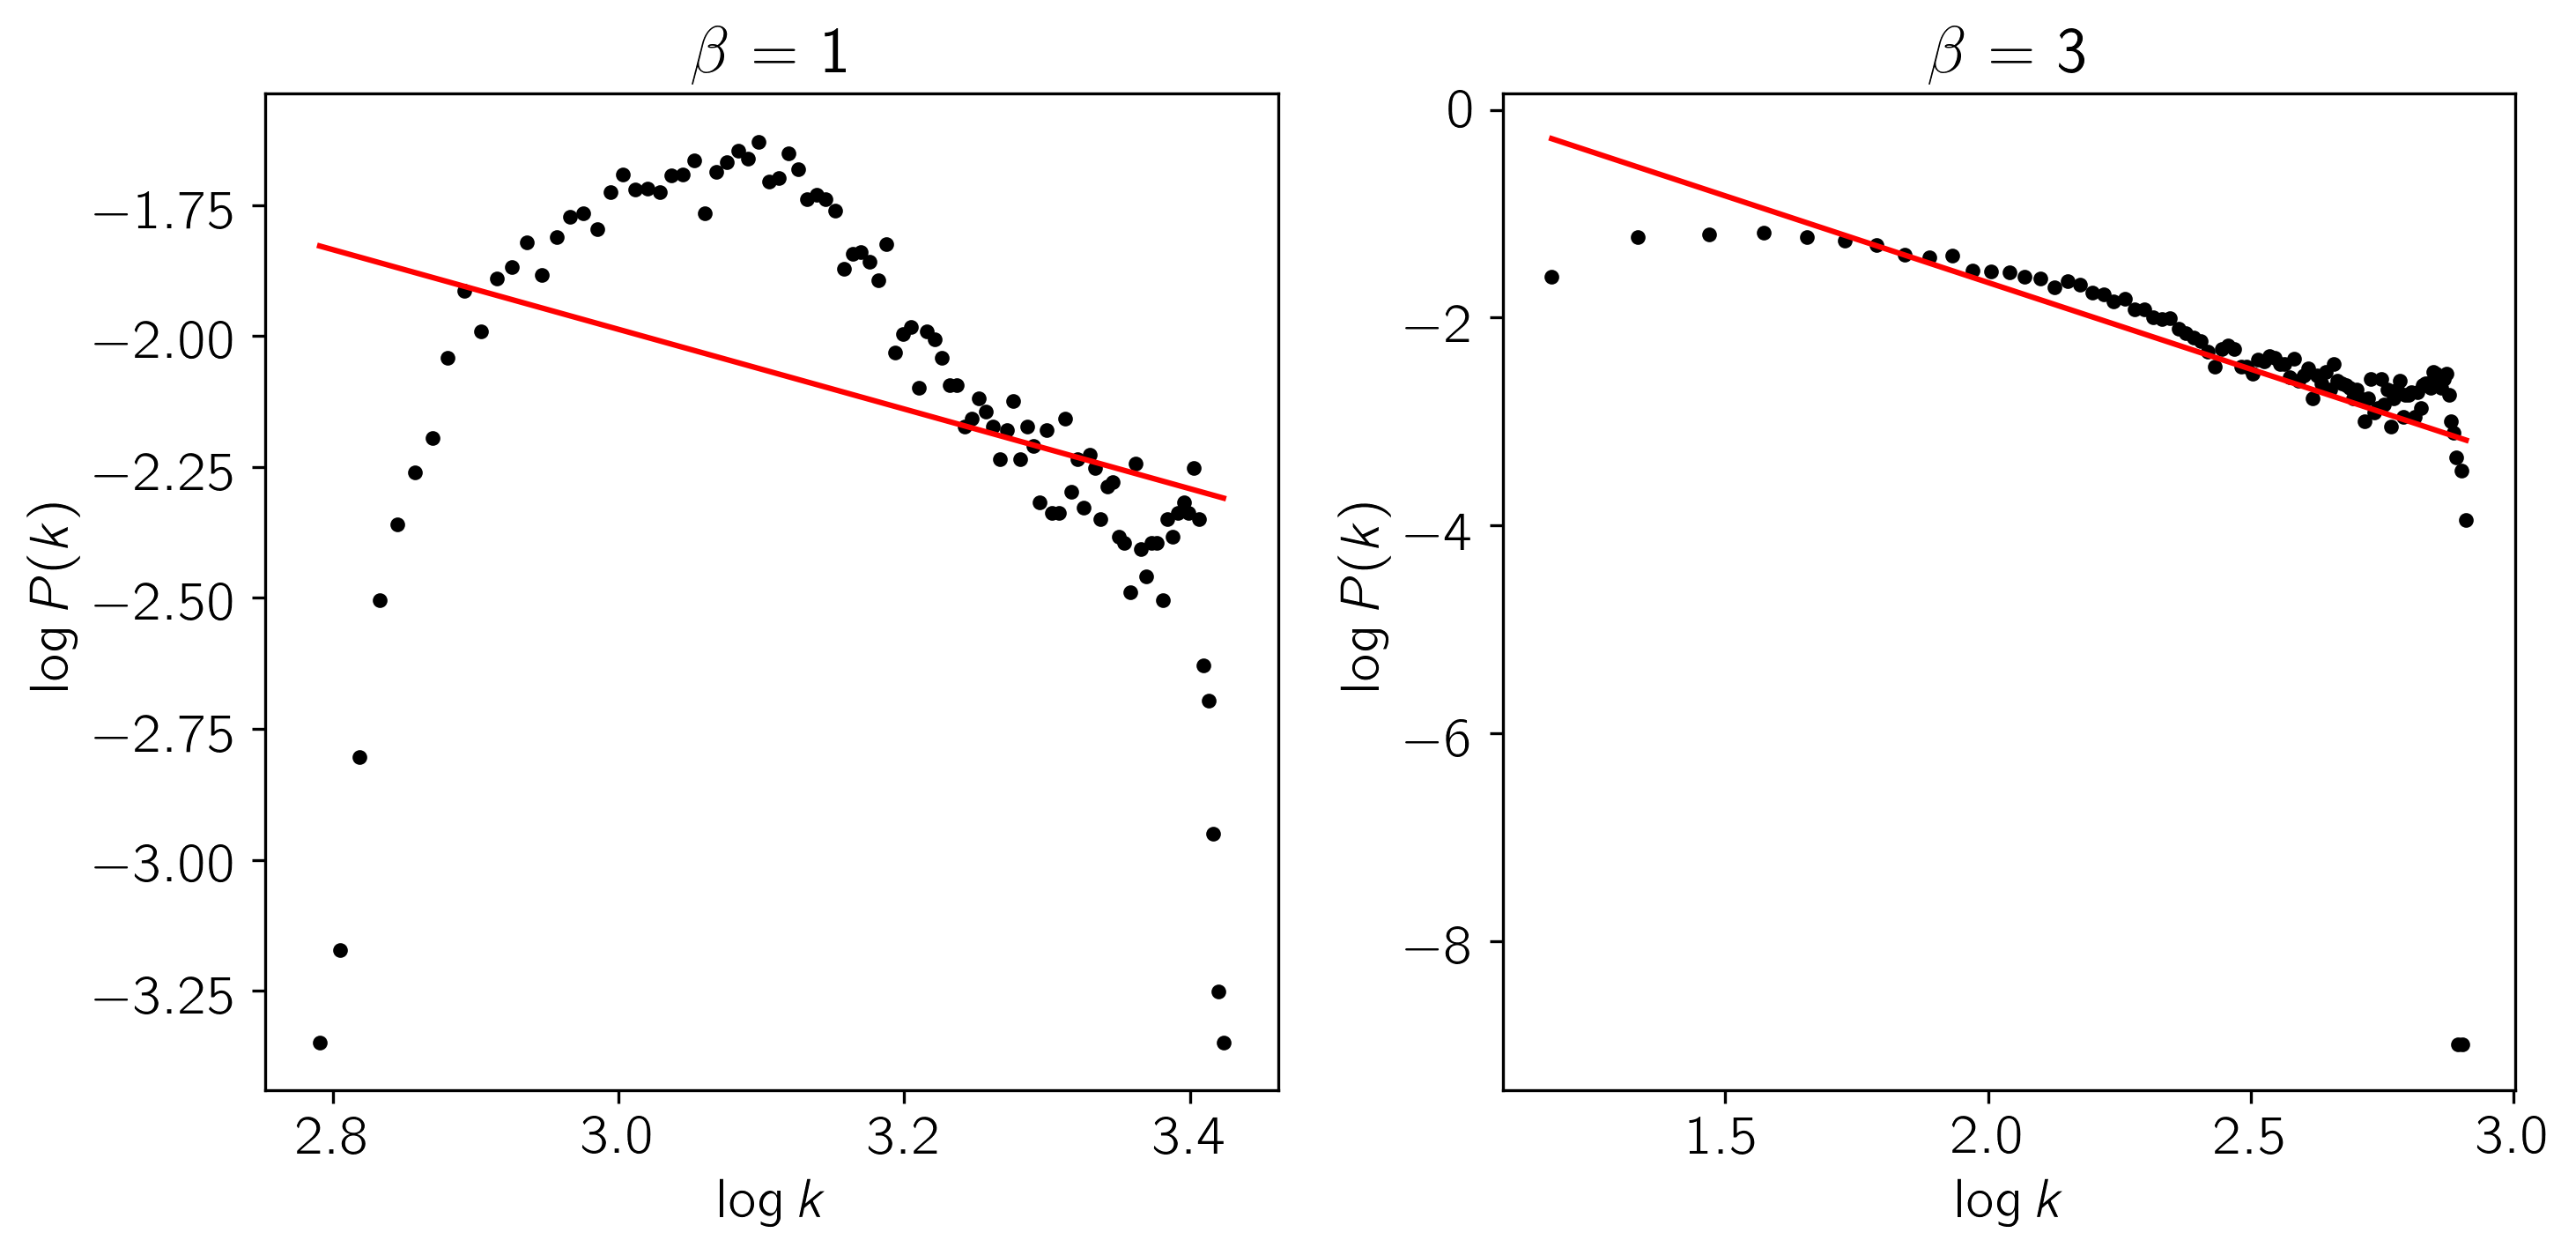
\includegraphics[clip,width=0.8\textwidth]{figures/figure2.png}
%  \caption{Degree distribution of $A$ (left) and $\hat{A}$ (right)}
%  \label{fig:beta}
%\end{figure}
%
%%overlapping percentage
%\begin{figure}[h!]
%  \centering
%    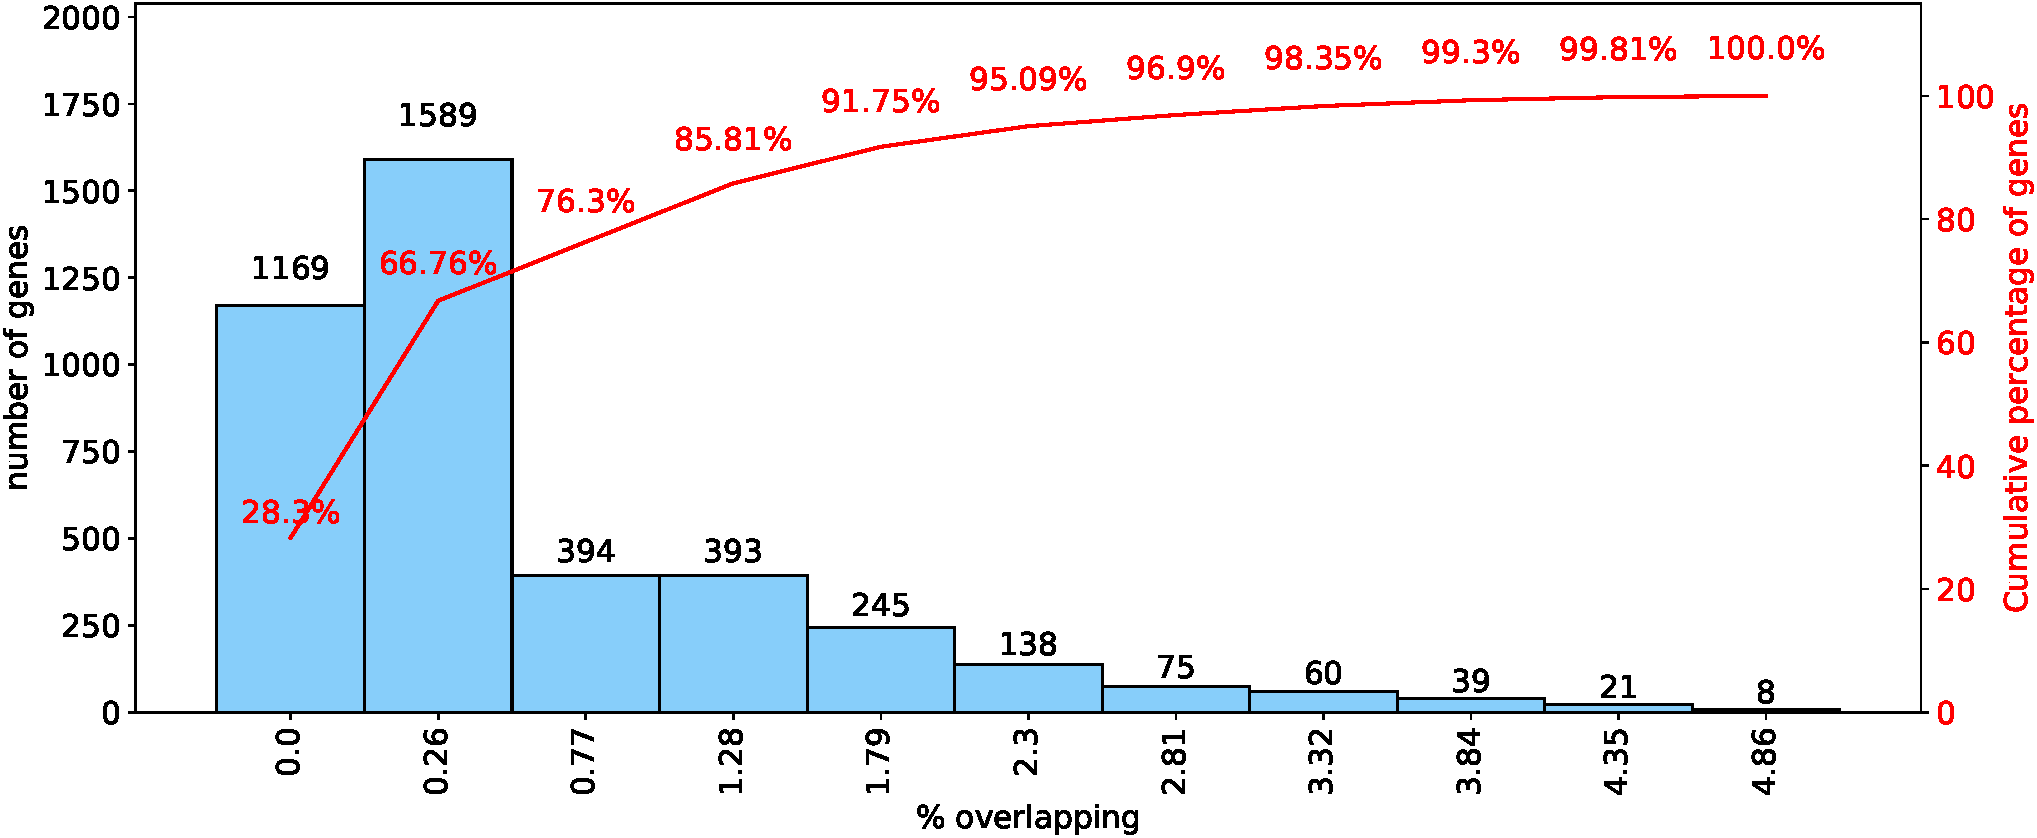
\includegraphics[clip,width=0.5\textwidth]{figures/figure3.png}
%  \caption{Overlapping percentage}
%  \label{fig:overlap}
%\end{figure}
%
%% boxplots
%\begin{figure}[h!]
%  \centering
%    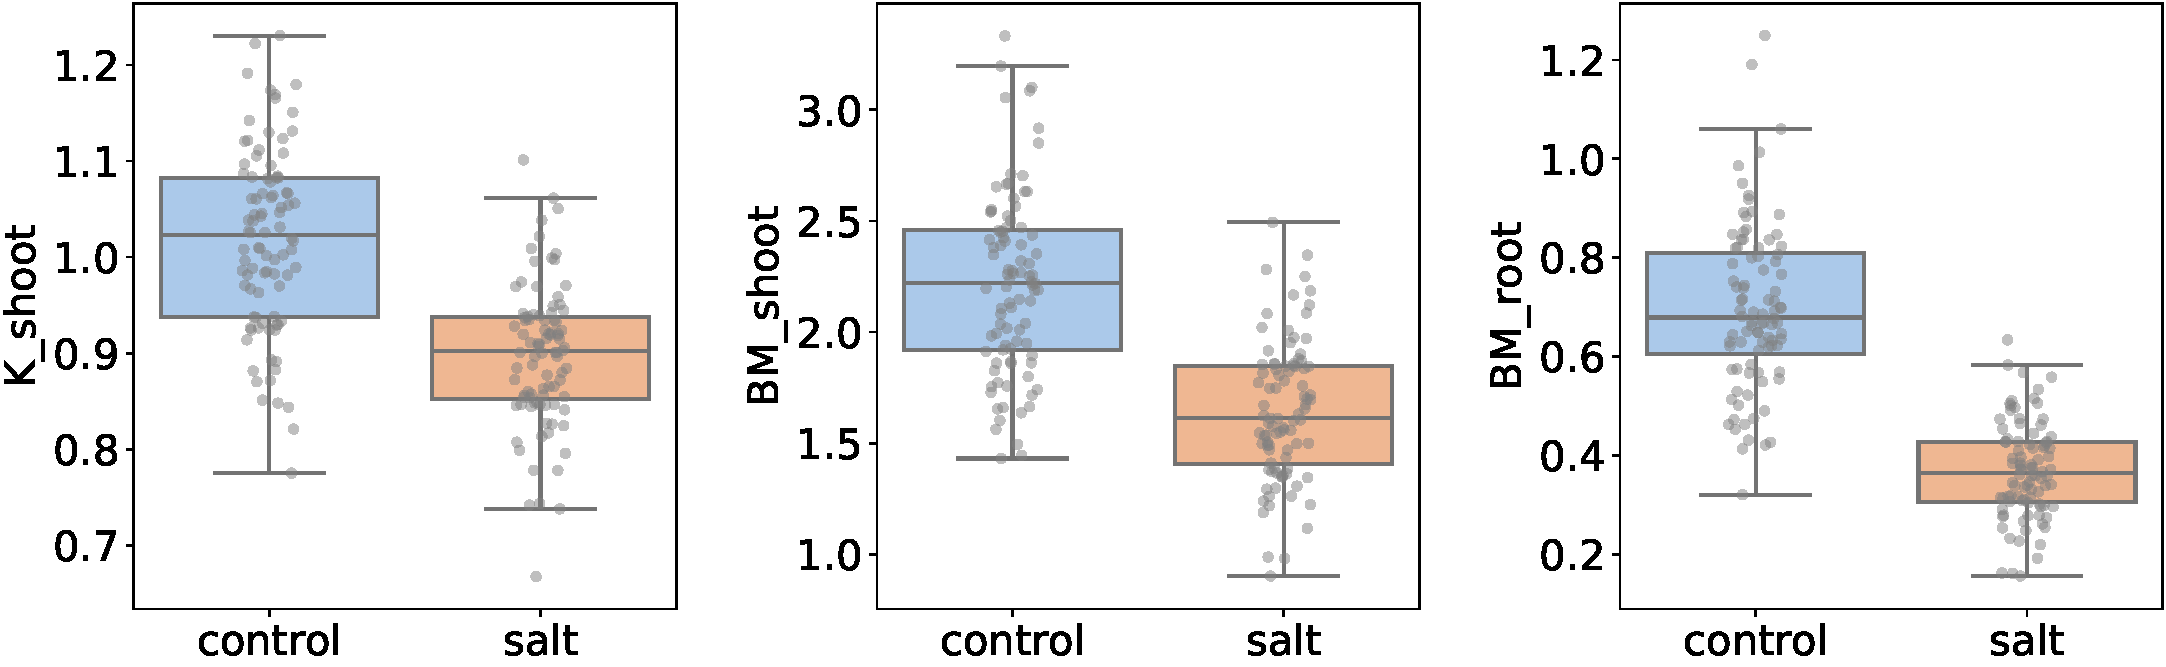
\includegraphics[clip,width=0.9\textwidth]{figures/figure4.png}
%  \caption{Phenotipic traits distribution under control and salt stress.}
%  \label{fig:pdata}
%\end{figure}
%
%\begin{figure}[h!]
%  \centering
%    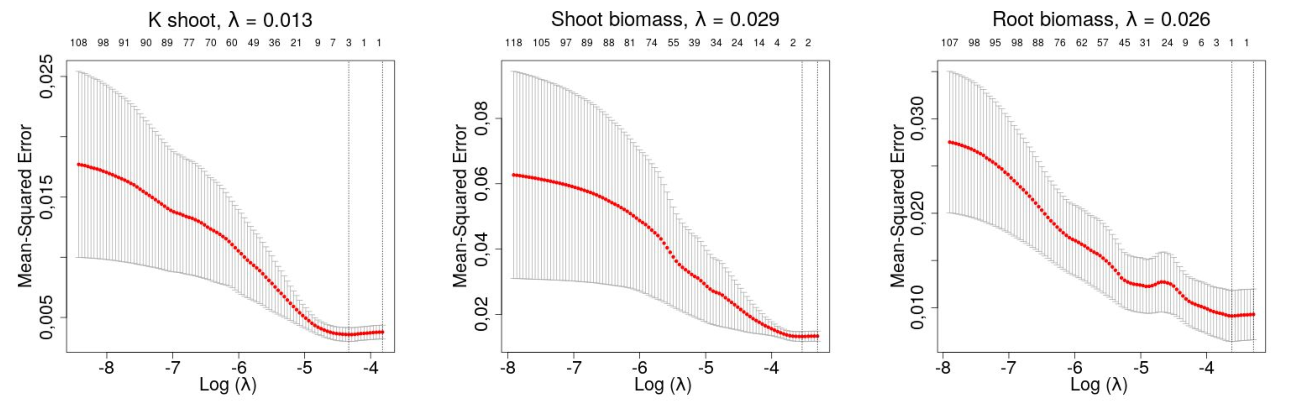
\includegraphics[clip,width=0.9\textwidth]{figures/figure5.pdf}
%  \caption{Cross-validation of the LASSO regularization parameter
%    $\lambda$, for each phenotypic trait.}
%  \label{fig:cross-val}
%\end{figure}
%
%\begin{figure}[h!]
%  \centering
%    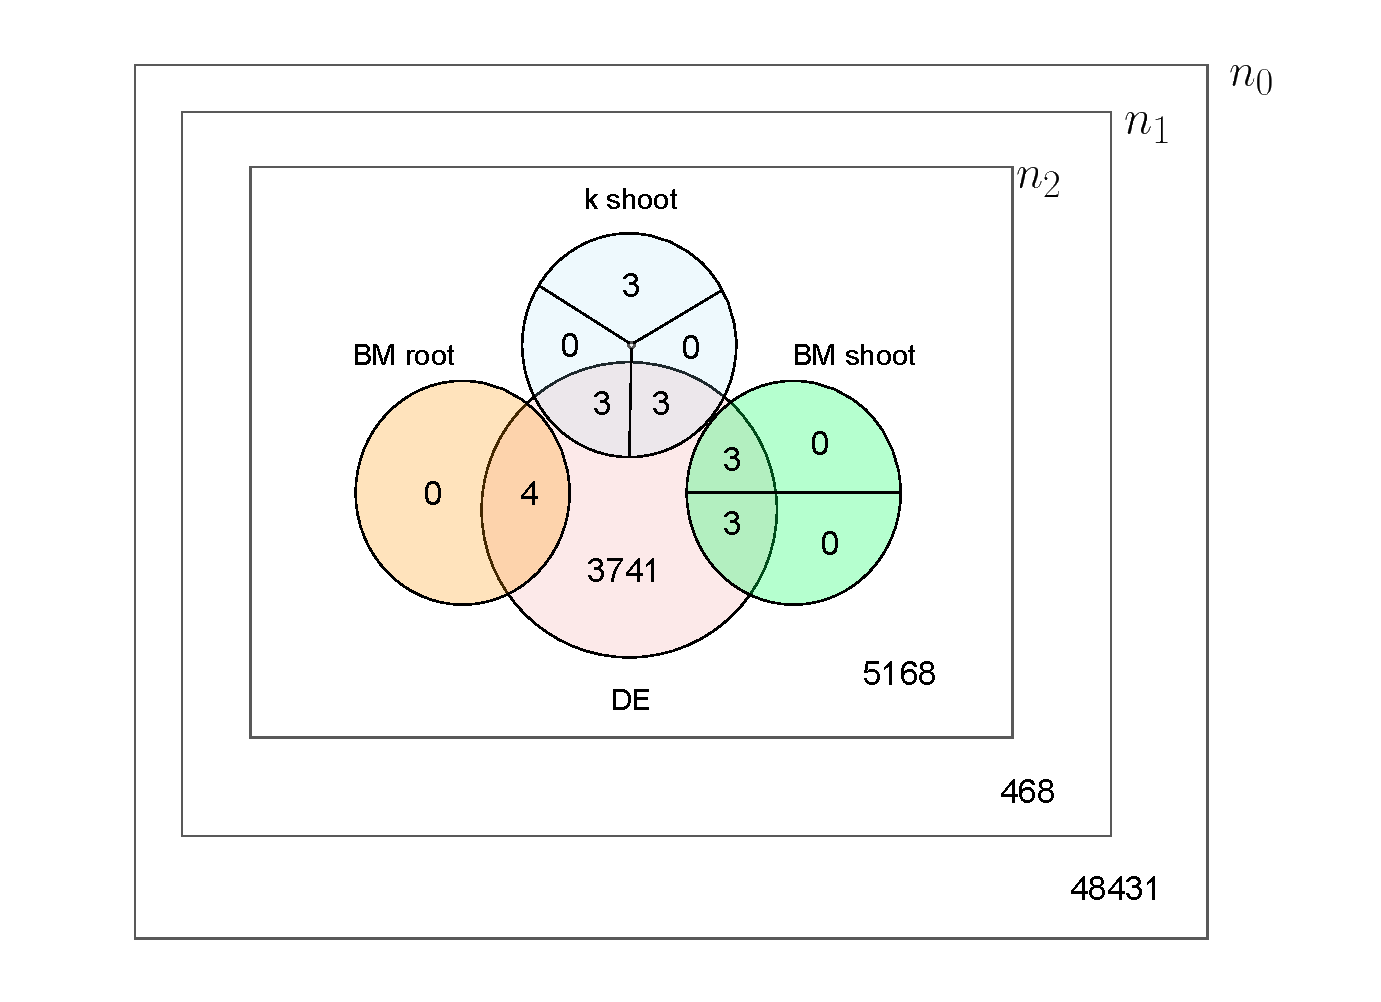
\includegraphics[clip,width=0.8\textwidth]{figures/figure6.pdf}
%   \caption[Venn diagram for the case study in rice]%
%   {Venn diagram representing the number of genes selected at
%    different stages of the proposed workflow for the case study in
%    rice.}
%  \label{fig:final_genes}
%\end{figure}
%
%% Figure 3d protein strucures
%\begin{figure}[hptb]
%  \centering
%    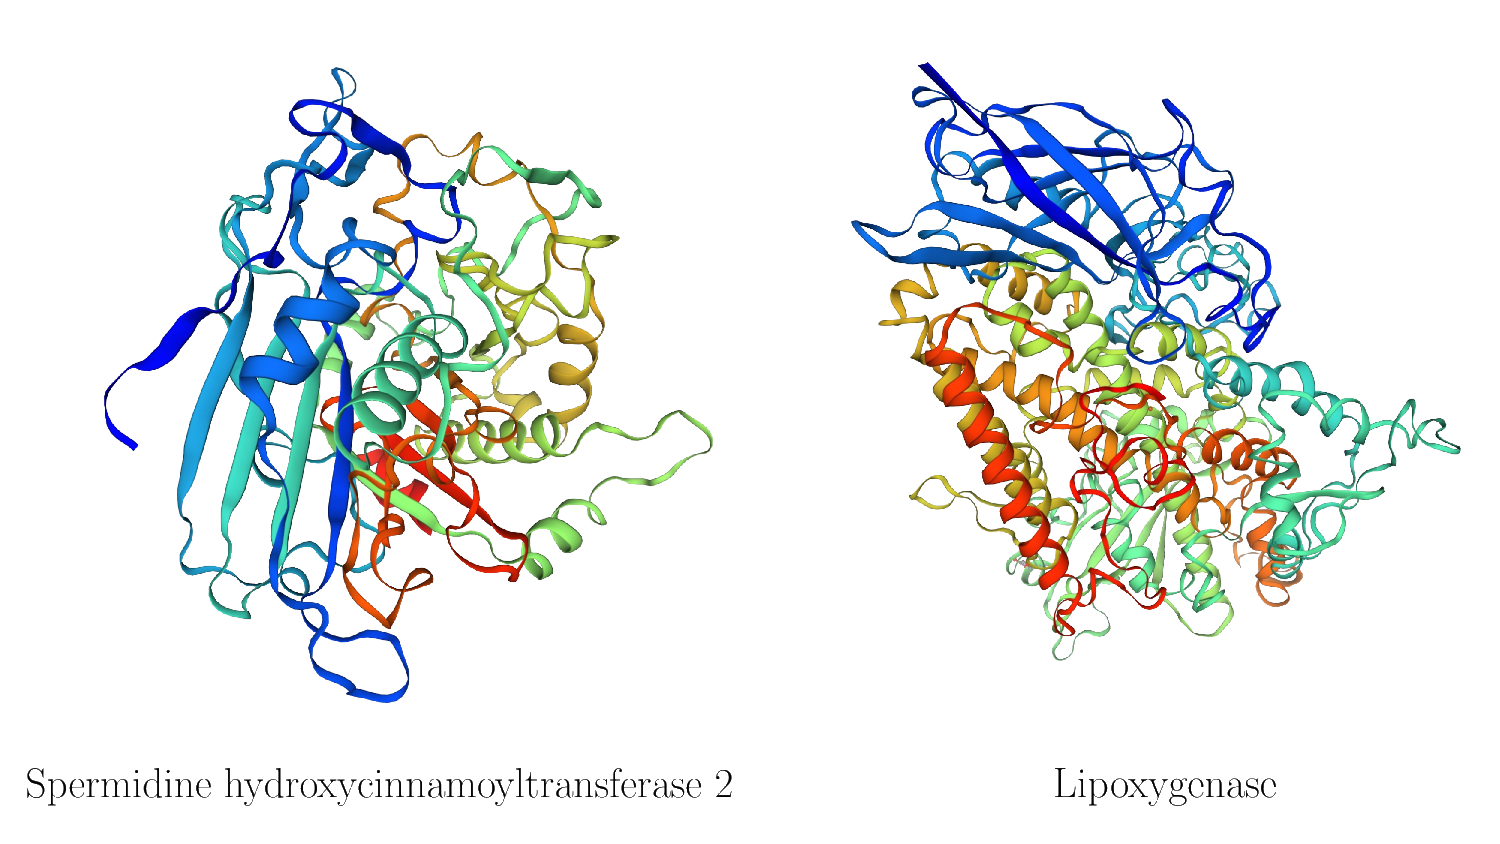
\includegraphics[clip,width=0.8\textwidth]{figures/figure7.pdf}
%  \caption{3D protein structure of named genes selected by LASSO, available from~\cite{szklarczyk2016string}.}
%  \label{fig:3d}
%\end{figure}

%%%%%%%%%%%%%%%%%%%%%%%%%%%%%%%%%%%
%%                               %%
%% Tables                        %%
%%                               %%
%%%%%%%%%%%%%%%%%%%%%%%%%%%%%%%%%%%

%% Use of \listoftables is discouraged.
%%
%\section*{Tables}
%\begin{table}[h!]
%\caption{Sample table title. This is where the description of the table should go}
%  \begin{tabular}{cccc}
%    \hline
%    & B1  &B2   & B3\\ \hline
%    A1 & 0.1 & 0.2 & 0.3\\
%    A2 & ... & ..  & .\\
%    A3 & ..  & .   & .\\ \hline
%  \end{tabular}
%\end{table}

%%%%%%%%%%%%%%%%%%%%%%%%%%%%%%%%%%%
%%                               %%
%% Additional Files              %%
%%                               %%
%%%%%%%%%%%%%%%%%%%%%%%%%%%%%%%%%%%

%\section*{Additional Files}
%  \subsection*{Additional file 1 --- Sample additional file title}
%    Additional file descriptions text (including details of how to
%    view the file, if it is in a non-standard format or the file extension).  This might
%    refer to a multi-page table or a figure.
%
%  \subsection*{Additional file 2 --- Sample additional file title}
%    Additional file descriptions text.

\end{backmatter}
\end{document}
